\documentclass[a4paper, 10pt]{article}
\usepackage[a4paper, margin=2cm]{geometry}
\usepackage[utf8]{inputenc}
\usepackage[T1]{fontenc}
\usepackage{graphicx}
\usepackage{wrapfig} % For wrapfigure environment
\usepackage{amsmath}
\usepackage{xcolor}
\usepackage{listings}
\usepackage{xcolor}
\usepackage{hyperref}
\usepackage{caption}
\usepackage{subcaption}
\usepackage{booktabs}
\usepackage{array}
\usepackage{etoolbox}
\usepackage{setspace} % line spacing control
\usepackage{parskip}  % No paragraph indentation
\usepackage{ragged2e} % Better left alignment
% \usepackage{floatrow}


\hypersetup{
    colorlinks=true,
    linkcolor=black,
    filecolor=magenta,      
    urlcolor=blue,
    pdftitle={Business-IT Alignment Dynamics},
    pdfpagemode=FullScreen,
}

\usepackage{minted}
\usemintedstyle{xcode} 
\usepackage{inconsolata} 

\setminted{
  frame=single,
  framesep=10pt,
  fontsize=\footnotesize,        
  linenos=false,  
  bgcolor=white,       
  breaklines=true,
  breakanywhere=true,
}

\definecolor{lightgray}{rgb}{0.95,0.95,0.95}

\lstdefinestyle{bashstyle}{
  backgroundcolor=\color{lightgray},
  basicstyle=\ttfamily\small,
  frame=single,
  framerule=0pt,
  rulecolor=\color{black},
  xleftmargin=1em,
  xrightmargin=1em,
  breaklines=true,
  postbreak=\mbox{\textcolor{gray}{$\hookrightarrow$}\space},
  showstringspaces=false,
  tabsize=2,
  language=bash
}

\title{Business-IT Alignment Dynamics: A Chaotic Systems Approach}
\author{Alessandro Aquilini}
\date{\today}

\begin{document}
\setstretch{1.1}
\raggedright 

\maketitle

\tableofcontents

\clearpage

\section{Introduction}
The project was developed for the \textbf{``Progetto di Ingegneria Informatica''} (PII) course at \textbf{Politecnico di Milano}, a \textbf{5 ECTS} course focused on hands-on projects in \textit{Computer Engineering}, covering software development, systems modeling, and data analysis.

I worked under the supervision of \textbf{Professor Fabrizio Amarilli} (Dept.\ of Management Engineering), who researches \textbf{business-IT strategic alignment}. Since complex systems often exhibit unpredictable long-term behavior, simulations are needed to study their dynamics. \newline
My task was to create a user-friendly platform for simulating his multi-parameter, discrete-time equation. The tool lets users adjust parameters, initial conditions, and simulation settings (like time steps and exploration ranges), providing outputs in visual diagrams and numerical tables.

The complete assignment track is available at: 
\href{https://pii.deib.polimi.it/a-platform-for-simulation-and-analysis-of-complex-systems/}{A Platform for Simulation and Analysis of Complex Systems}.

The main result is a \textbf{Python Notebook} with four embedded interactive tools powered by the Matplotlib engine for studying the model. Namely:

\begin{enumerate}
    \item \textit{Time Evolution Simulation}: Observe alignment trends over time
    \item \textit{Cobweb plot}: Identify periodic and chaotic behavior.
    \item \textit{Phase Portrait Analysis}: Visualize stability and equilibrium points
    \item \textit{Bifurcation Diagram} and \textit{Lyapunov exponent}: Explore chaotic regimes and parameter sensitivity
\end{enumerate}

More details can be found in the \hyperref[sec:results]{results} section.

On a final note, I took a keen interest in studying the mathematics behind the fascinating field of "chaotic phenomena". 
To enrich the user experience, I thought it would be helpful to include some explanations and add few compelling cases.

\subsubsection*{Why a Python Notebook fits this project?}

\begin{itemize}
    \item \textit{User-friendly}: Even non-coders can tweak parameters via sliders and see instant results
    \item \textit{Shareable}: Runs anywhere (Jupyter, VS Code, Google Colab) with no setup headaches
    \item \textit{Explanatory}: Combines code, visuals, and text explanations in one place
\end{itemize}

\section{User Requirements}
\subsection{Target Audience}
This interactive notebook is designed for anyone interested in Business-IT alignment dynamics. \\
It also serves as template for modeling other complex dynamics that use discrete time equations in the form of $x_{t+1} = x_t + \Delta(t, \text{*args})$. The user just needs to apply a few minor customization to the code.

\subsection{Getting Started}
\subsubsection{Installation}
\begin{enumerate}
    \item Clone the repository:
    \begin{lstlisting}[style=bashstyle]
git clone https://github.com/Kinshale/pii.git
cd pii
    \end{lstlisting}

    \item Install required packages:
    \begin{lstlisting}[style=bashstyle]
pip install numpy matplotlib ipywidgets
    \end{lstlisting}
\end{enumerate}

\subsubsection{Running the Notebook}
Choose your preferred environment:
\begin{itemize}
	\item \textbf{Local Jupyter}: Launch Jupyter Notebook and open \texttt{pii.ipynb}
	\item \textbf{VS Code}: Open the notebook with Jupyter extension
	\item \textbf{Google Colab}:
	      \begin{enumerate}
		      \item Visit \url{https://colab.research.google.com}
		      \item Select "GitHub" tab and paste the notebook URL
		      \item Or open the cloned one
	      \end{enumerate}
\end{itemize}

For optimal experience:
\begin{itemize}
	\item Start with default parameters to observe baseline behavior
	\item Modify one parameter at a time to understand its effect
	\item Use the bifurcation tool to identify chaotic parameter regions
	\item Read the markdown cells
\end{itemize}

\subsection{Customizing the Notebook}
The provided notebook is designed as a \textbf{template} for simulating \textit{any} discrete-time dynamical system of the form:

\begin{equation}  
x_{t+1} = x_t + \Delta(t, \theta_1, \theta_2, \dots)  
\end{equation}

where \(\Delta(\cdot)\) is a user-defined function and \(\theta_i\) are parameters. To adapt it for a new equation, follow these steps:

\subsubsection*{1. Define the Delta Function}
Replace the \texttt{delta()} function in the \textbf{Core Code} section with your custom \(\Delta(\cdot)\). For example, to simulate the logistic map:

\begin{minted}{python}
def delta(x, r):
    return r * x * (1 - x)  # Logistic growth
\end{minted}

\vspace{-1.5em}

\subsubsection*{2. Update Parameters}
Modify the \texttt{PARAMETERS} dictionary to include your equation's parameters (e.g., growth rate \(r\)):

\begin{minted}{python}
PARAMETERS = {
    "r": {
        "default": 3.2,
        "description": "Growth rate",
        "range": {"min": 1.0, "max": 4.0, "step": 0.01}
    },
    ...  # Keep other parameters (x0, steps) unchanged
}
\end{minted}

\vspace{-1.5em}

\subsubsection*{3. Adjust Visualization}
Update the \textit{ipywidgets} sliders accordingly and the built-in tools will automatically adapt to new equations.

\clearpage
\section{Model Description}
\subsection{Core Equation}
The alignment dynamics are governed by:

\begin{equation}
	x_{t + 1} = x_t + A(x_t) - B(x_t)C(x_t)
\end{equation}

Where:
\begin{itemize}
	\item $x_t$: Percentage of dissatisfied users (misalignment proxy)
	\item $A(x_t)$: Environmental pressure effect
	\item $B(x_t)$: IT department efficacy
	\item $C(x_t)$: Organizational adaptability
\end{itemize}

\subsection{Component Functions}
\begin{align}
	A(x_t) & = d(1 - x_t)                                                                     \\
	B(x_t) & = \frac{a x_t (1 - x_t)^g}{1 + a h x_t}                                          \\
	C(x_t) & = \frac{1}{1 + z^s} \quad \text{where} \quad z = \frac{r (1 - x_t)}{x_t (1 - r)}
\end{align}

\subsection{Parameter Definitions}
\begin{table}[h]
	\centering
	\caption{Model Parameters and Ranges}
	\begin{tabular}{llll}
		\toprule
		\textbf{Parameter} & \textbf{Description}       & \textbf{Range} & \textbf{Default} \\
		\midrule
		$x_0$              & Initial misalignment       & [0.01, 0.99]   & 0.3              \\
		$d$                & Environmental dynamicity   & [0.1, 2]      & 0.5              \\
		$a$                & IT department efficacy     & [0.1, 10]      & 2                \\
		$h$                & IT system rigidity         & [0.1, 5]       & 1                \\
		$g$                & IT investment propensity   & [0.1, 5]       & 1                \\
		$r$                & Action threshold           & [0.01, 0.99]   & 0.3              \\
		$s$                & Organizational flexibility & [1, 10]        & 3                \\
		\bottomrule
	\end{tabular}
\end{table}

\subsection{Interpretation}
Let's take a deeper look at our equation:

\begin{equation}
	x_{t + 1} = x_t + \underbrace{A(x_t)}_{\text{Environmental Pressure}} - \underbrace{B(x_t)C(x_t)}_{\text{Recovery Mechanism}}
\end{equation}

\begin{description}
	\item[$x_t$ \textendash\ Alignment] Measures the percentage of dissatisfied users at time $t$:
		\begin{itemize}
			\item $0 \rightarrow$ Complete satisfaction (perfect alignment)
			\item $1 \rightarrow$ Utter dissatisfaction (total misalignment)
		\end{itemize}

	\item[$A(x_t)$ \textendash\ Environmental Pressure:] Increases misalignment due to external factors, representing how competitive environments and technological changes increase dissatisfaction.

	\item[$B(x_t) \cdot C(x_t)$ \textendash\ Recovery Mechanism:] Reduces misalignment through:
		\begin{itemize}
			\item $B(x_t)$: IT department's effectiveness.
			\item $C(x_t)$: Organization's adaptability.
		\end{itemize}
\end{description}

\subsection{Parameter Analysis}
Full interactive simulation available at: \url{https://www.desmos.com/calculator/qdendm1pfg}

\subsubsection{Environmental Pressure Function}
\begin{equation}
	A(x_t) = d(1 - x_t)
\end{equation}

Forms a line passing through $(1, 0)$ with slope $-d$.
\begin{itemize}
	\item \textbf{$d$ (dynamicity)}: Fast changing industries (e.g., a tech startup) have a competition/innovation that rapidly renders old IT systems obsolete.
	\item \textbf{$1 - x_t$}: As misalignment grows, environmental pressure has less "room" to worsen things.
\end{itemize}

\subsubsection{IT Department Efficacy}
\begin{equation}
	B(x_t) = \frac{a x_t (1 - x_t)^g}{1 + a h x_t}
\end{equation}

This looks like a function that peaks at some $x_a$ and then tapers off.

\begin{itemize}
	\item \textbf{a (IT efficacy)}: an higher a can more effectively reduce misalignment.
	\item \textbf{x (current misalignment)}: the more misalignment exists, the more opportunity/pressure there is for IT to act.
	\item \textbf{$(1 - x_t)^g$ (Diminishing Returns)}: as satisfaction improves, the IT department's impact diminishes.
	      \begin{itemize}
		      \item I haven't understood g.
	      \end{itemize}
	\item \textbf{$1 + ahx_t$ (Saturation)}: even if IT is highly capable (a >> 1), inflexible systems (h >> 1) limit its efficacy.
\end{itemize}



\subsubsection{Organizational Adaptability}
\begin{equation}
	C(x_t) = \frac{1}{1 + z^s} \quad \text{where} \quad z = \frac{r (1 - x_t)}{x_t (1 - r)}
\end{equation}

This is a \textbf{sigmoid} function in disguise. Sigmoids are exploited for modeling "threshold behaviors".

\begin{itemize}
	\item \textbf{r (activation threshold)}: below r, the organization resists to change ($C(x) \rightarrow 0$). But when misalignment crosses a certain threshold adaptability kicks in.
	\item \textbf{s (flexibility)}: higher s make the sigmoid steeper (sharper transition from resistance to adaptation).
\end{itemize}

\begin{figure}[h]
	\centering
	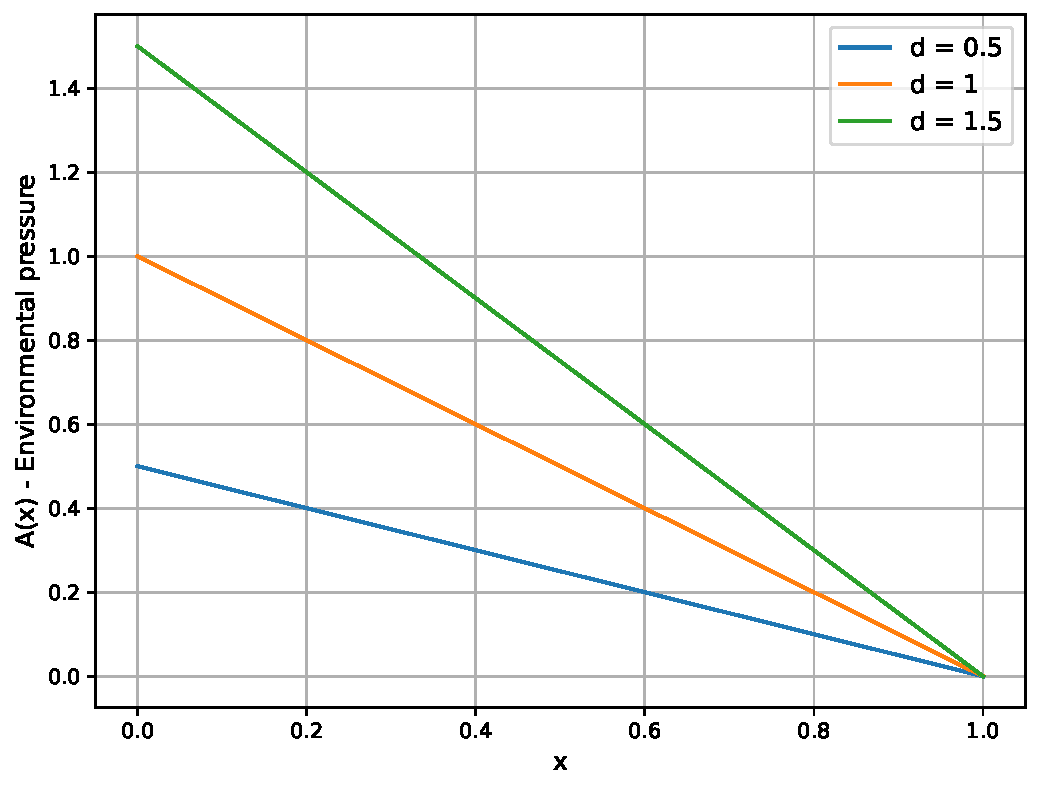
\includegraphics[width=0.5\textwidth]{../images/params/A(x).pdf}
	\caption{Environmental pressure function for varying $d$ values}
\end{figure}

\begin{figure}[h]
	\centering
	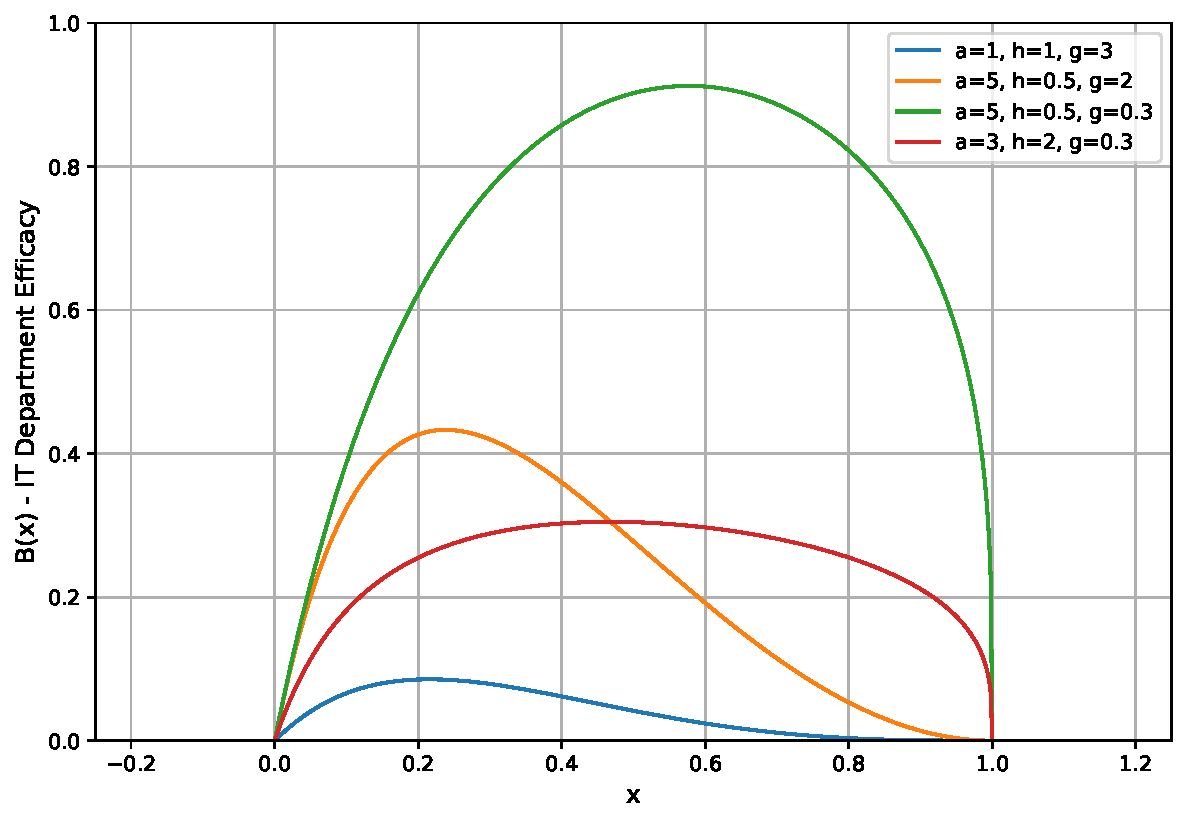
\includegraphics[width=0.75\textwidth]{../images/params/B(x).pdf}
	\caption{IT efficacy function showing the effect of parameters $a$, $h$, and $g$}
\end{figure}

\begin{figure}[h]
	\centering
	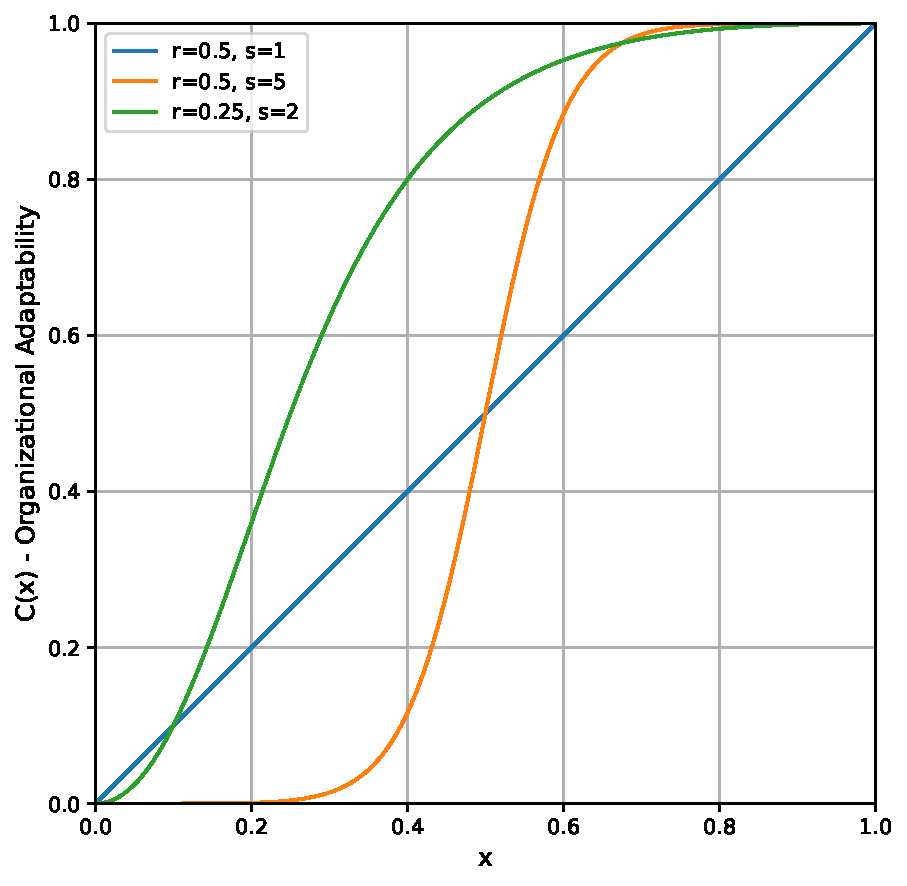
\includegraphics[width=0.70\textwidth]{../images/params/C(x).pdf}
	\caption{Organizational adaptability function demonstrating threshold behavior}
\end{figure}

\clearpage
\section{Implementation}
\subsection{Technological Stack}
\begin{itemize}
	\item Python 3.10.12 (managed via Conda)
	\item Jupyter Notebook for interactive exploration, with markdown explanations attached
	\item Core dependencies (Python Libraries)
	      \begin{itemize}
		      \item NumPy for numerical computations
		      \item Matplotlib for visualization graphs
		      \item ipywidgets for parameter sliders
	      \end{itemize}
\end{itemize}

\subsection{Key lines of code}
\subsubsection{Simulating the equation}
The equation is hardcoded:
\begin{minted}{python}
def A(x, d):
    return d * (1 - x)

def B(x, a, h, g):
    return (a * x * (1 - x) ** g) / (1 + a * h * x)

def C(x, r, s):
    if x == 0:  # Avoid division by zero
        return 0
    z = (r * (1 - x)) / (x * (1 - r))
    return 1 / (1 + z ** s)

def delta(x, d, a, h, g, r, s):
    return A(x, d) - B(x, a, h, g) * C(x, r, s)

def simulate(x0, d, a, h, g, r, s, steps=100):
    x = np.zeros(steps)
    x[0] = x0
    for t in range(steps - 1):
        x[t + 1] = np.clip(x[t] + delta(x[t], d, a, h, g, r, s), 0, 1)
\end{minted}
\vspace{-3em}
\subsubsection{Long term behavior}
Here is the key logic behing classifing the equation:

\begin{minted}{python}
x = simulate(x0, d, a, h, g, r, s, steps)

last_values = x[-10:]

if np.std(last_values) < 0.001:  # Stable state
final_val = np.mean(last_values)
if final_val < 0.1:
    return x, "ALIGNED"
elif final_val > 0.9:
    return x, "MISALIGNED"
else:
    return x, "PARTIAL_ALIGNMENT"
else:  # Dynamic state
if len(np.unique(np.round(last_values, 2))) > 3:
    return x, "CHAOTIC"
else:
    return x, "OSCILLATING"
\end{minted}
\vspace{-3em}

\subsubsection{Lyapunov exponent}
The implementation for computing the Lyapunov exponent:

\begin{minted}{python}
def compute_lyapunov_exponent(x0=0.3, epsilon=1e-8, steps=50, **kwargs):
    x = simulate(x0=x0, steps=steps, **kwargs)
    x_perturbed = simulate(x0=x0 + epsilon, steps=steps, **kwargs)

    separation = np.abs(x_perturbed - x)

    valid_indices = separation > 0
    if np.sum(valid_indices) < 2:
        return 0

    t = np.arange(steps)[valid_indices]
    log_sep = np.log(separation[valid_indices])

    # Perform linear regression
    coeffs = np.polyfit(t, log_sep, 1)
    lyapunov_exponent = coeffs[0]

    return lyapunov_exponent
\end{minted}
\vspace{-3em}

\subsubsection{Bifurcation Analysis}
The chaotic regime detection algorithm:

\begin{minted}{python}
def bifurcation_analysis(param, p_min, p_max, fixed_params, n_points=500):
    param_values = np.linspace(p_min, p_max, n_points)
    n_transient = 200  # Skip initial transient
    n_samples = 100    # Points to plot per parameter
    
    for p in param_values:
        params = fixed_params.copy()
        params[param] = p
        
        x = 0.3  # Initial value
        # Burn-in phase
        for _ in range(n_transient):
            x = np.clip(x + delta(x, **params), 0, 1)
        
        # Sample stable points
        x_vals = []
        for _ in range(n_samples):
            x = np.clip(x + delta(x, **params), 0, 1)
            x_vals.append(x)
        
        plt.plot([p]*n_samples, x_vals, 'k.', markersize=0.5)
\end{minted}
\vspace{-3em}

\subsection{Numerical Considerations}
\begin{itemize}
	\item State clipping ensures $x_t \in [0,1]$ remains meaningful
	\item All floating-point operations use NumPy's float64 precision
	\item The bifurcation analysis skips 200 transient iterations to focus on long-term behavior
\end{itemize}

\clearpage
\section{Results}
\label{sec:results}
\subsection{Interactive Tools}
The notebook provides four powerful ways to explore alignment dynamics. 
You can adjust the parameters of the equations through \textbf{sliders}, interact with \textbf{dropdowns} and even select \textbf{tabs}. The diagram will update in real-time.

\begin{figure}[h!]
    \centering
    \begin{subfigure}{0.45\textwidth}
        \centering
        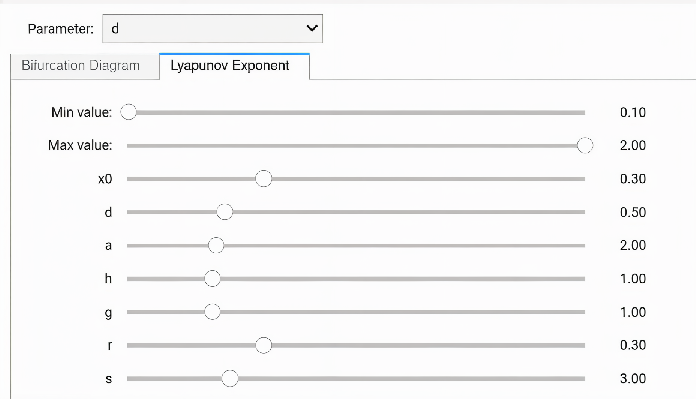
\includegraphics[width=\linewidth]{../images/results/slid-1.pdf}
        \label{fig:sliders1}
    \end{subfigure}
    \hfill
    \begin{subfigure}{0.45\textwidth}
        \centering
        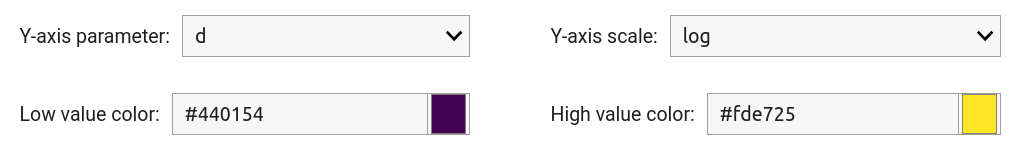
\includegraphics[width=\linewidth]{../images/results/slid-2.png}
        \label{fig:sliders2}
    \end{subfigure}
    \caption{(Blurred) Interactive sliders}
    \label{fig:side_by_side}
\end{figure}

{\footnotesize \textbf{Note:} I spent a couple of hours trying to get high quality screenshots, but it's impossible. So run the notebook to see the sliders.
}

\subsubsection{Time Evolution Simulation}
The time evolution simulation displays how alignment changes over successive iterations.
You can also tweak the initial condition ($x_0$) and the number of iterations. 

\begin{figure}[h]
	\centering
	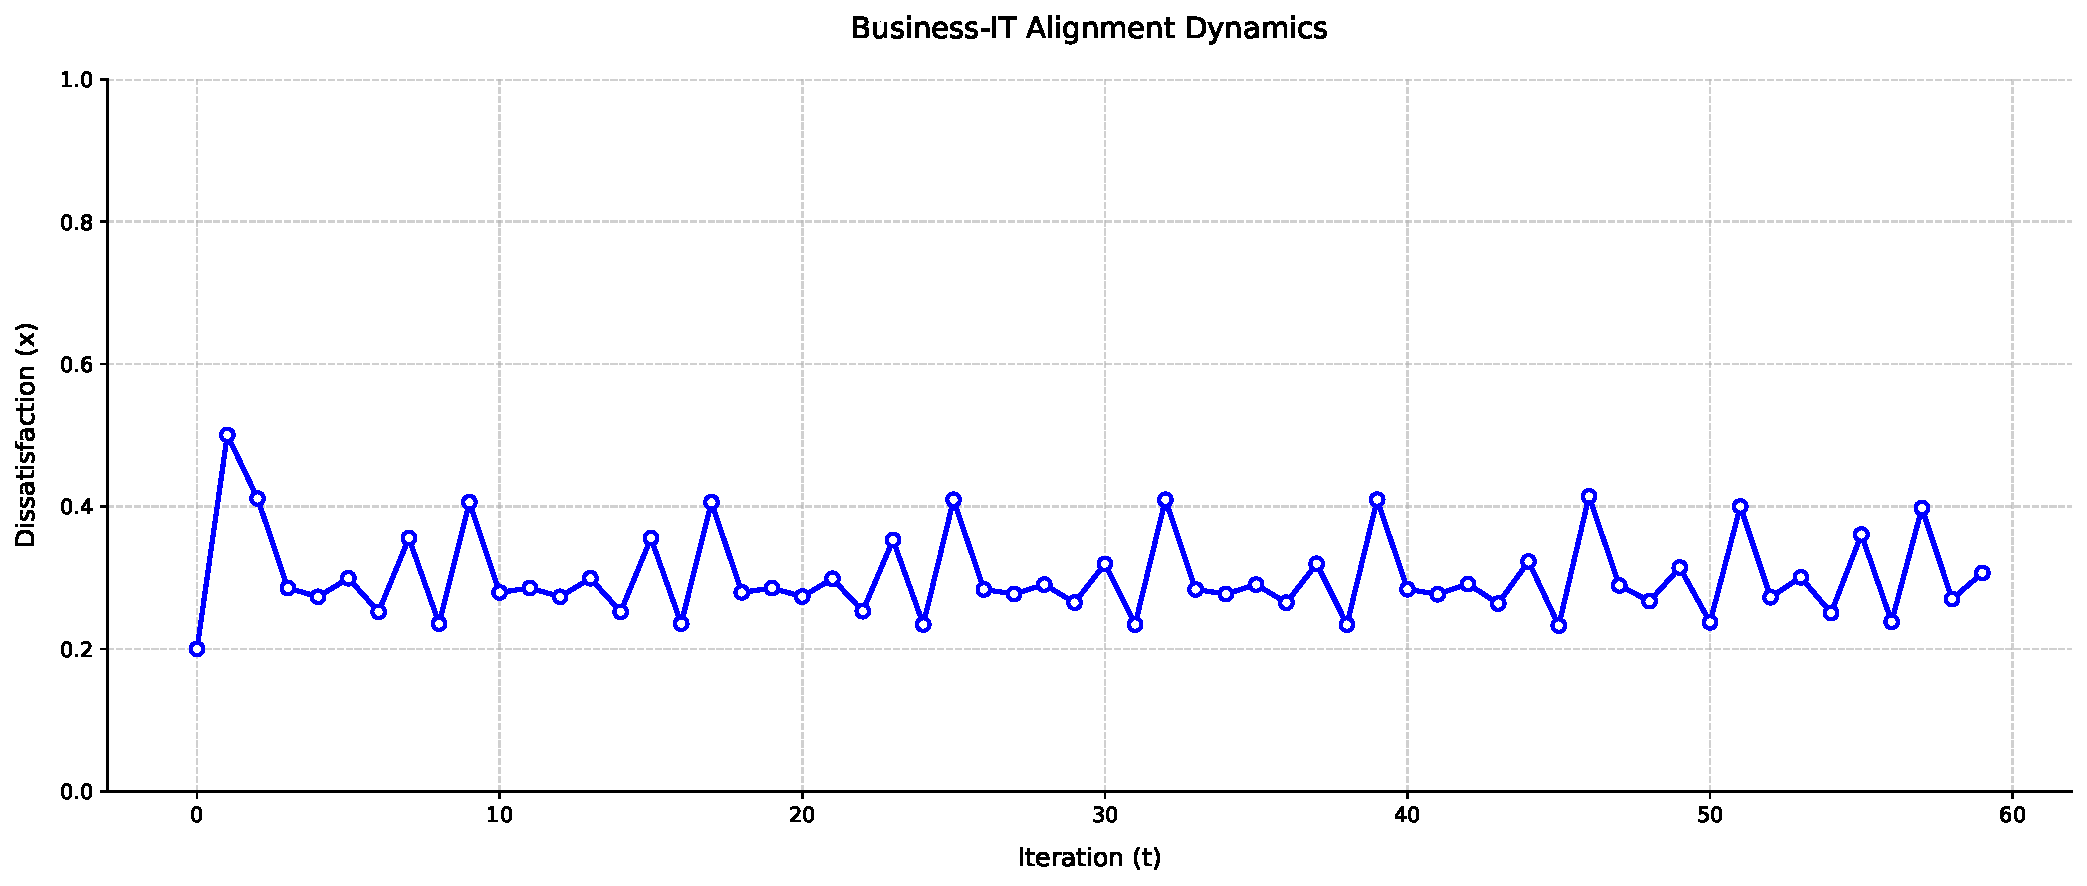
\includegraphics[width=1\textwidth]{../images/results/time-evolution.pdf}
	\caption{Time evolution showing chaotic behaviour ($d = 0.5$, $a = 6$, $h = 0.4$, $g = 2$, $r = 0.25$, $s = 5$)}
	\label{fig:time_sim}
\end{figure}

\subsubsection{Cobweb Plot}
A cobweb plot visualizes the dynamics of iterative functions. 
It traces the evolution of a sequence by stepping between the function curve and the identity line $y = x$. This diagram helps analyze stability, convergence, or divergence of fixed points in dynamical systems. 

In a Lémeray (cobweb) diagram, \textit{stable fixed points} appear as shrinking staircases or inward spirals, while unstable ones grow outward.
As the system evolves, periodic orbits emerge as closed shapes, like rectangles or loops, that repeat over multiple steps.
In contrast, chaotic behavior fills a region densely with no repeating pattern, indicating sensitive dependence on initial conditions.
All fixed points can be identified where the function curve intersects the diagonal $y = x$.

\begin{figure}[H]
	\centering
	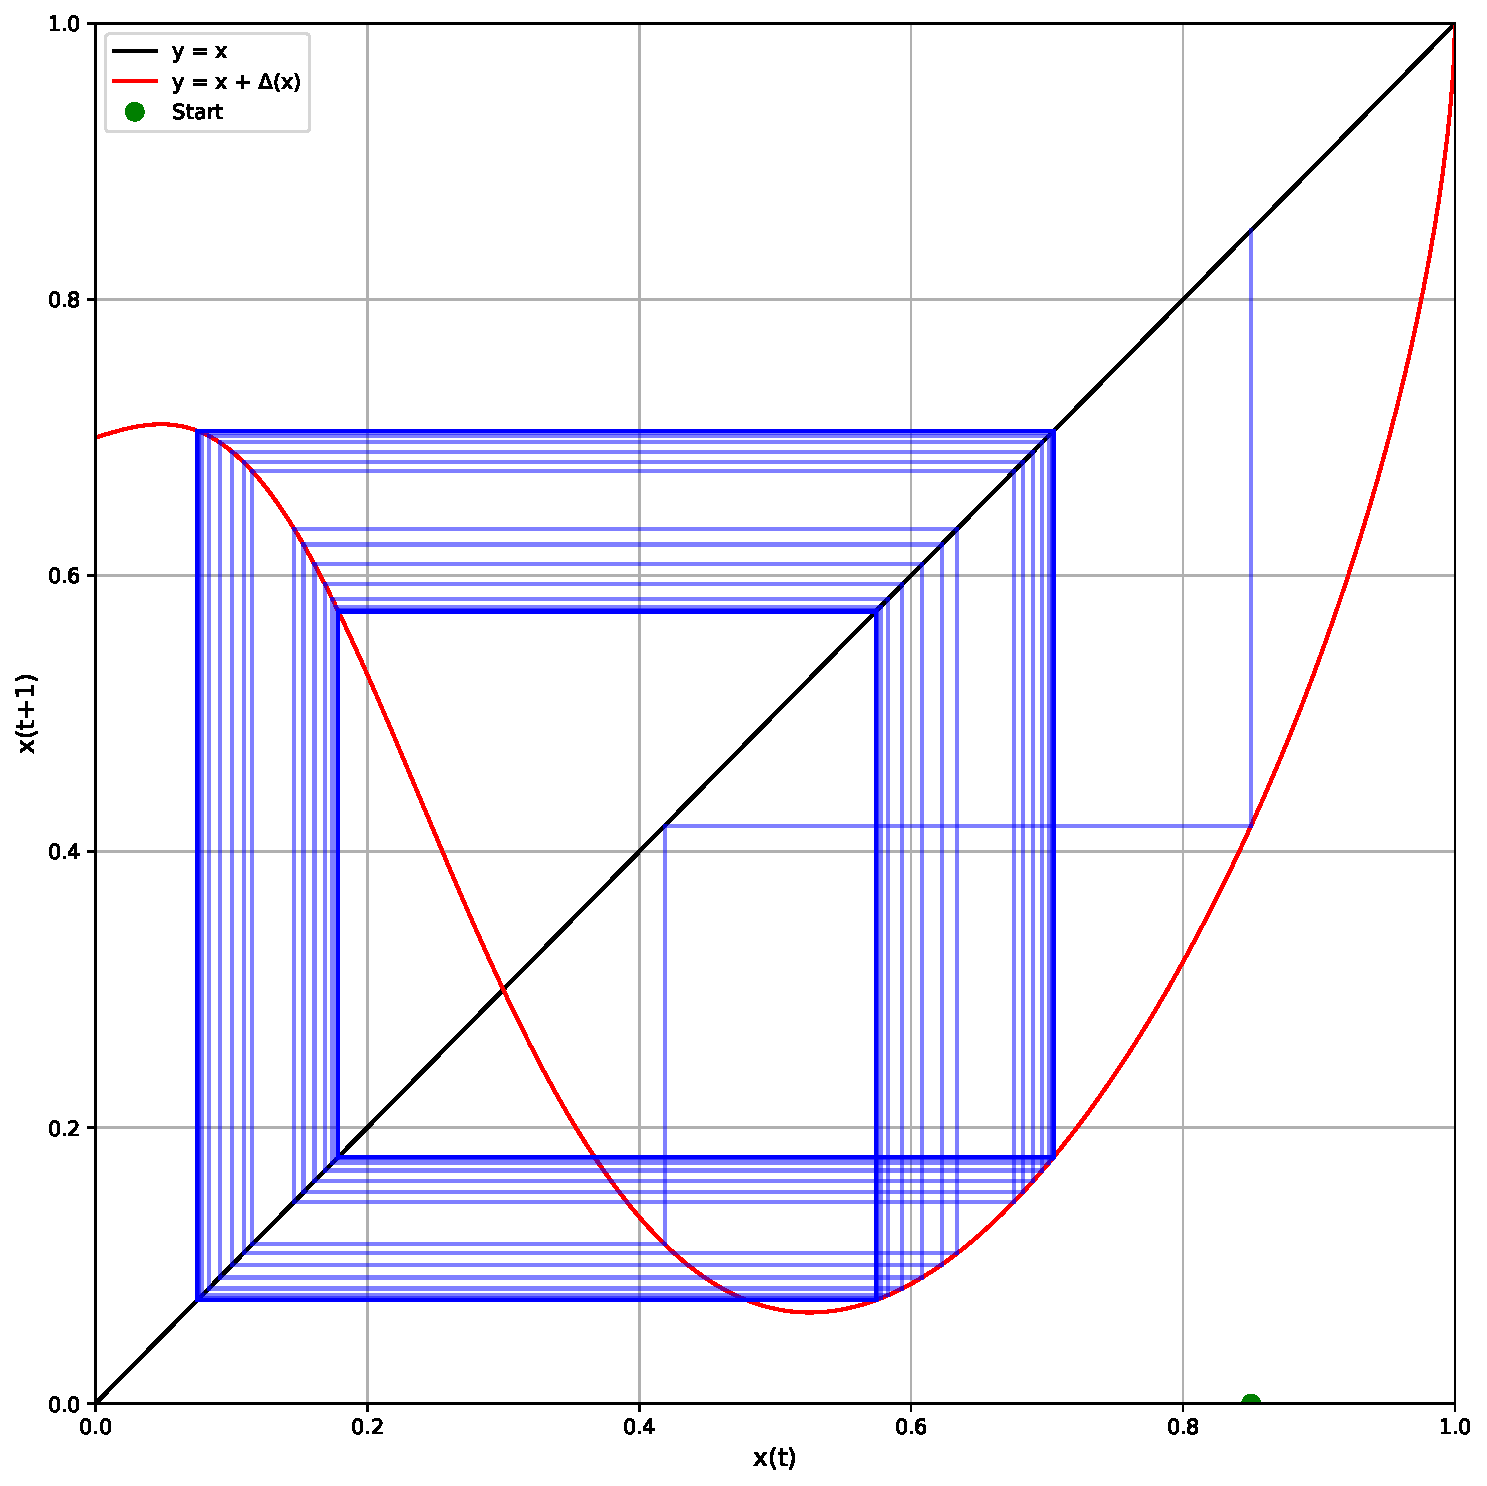
\includegraphics[width=0.7\textwidth]{../images/results/cobweb.pdf}
	\caption{Cobweb plot ($x_0 = 0.85$, $d = 0.7$, $a = 5$, $h = 0.36$, $g = 0.6$, $r = 0.25$, $s = 2$)} % cobweb_plot(0.85, 0.7, 5, 0.36, 0.60, 0.25, 2, 100)
	\label{fig:cobweb_plot}
\end{figure}

\subsubsection{Phase Portrait Analysis}
The phase portait examines the system's underlying dynamics through multiple visual cues. Arrow directions indicate whether misalignment tends to increase or decrease at each state point, while a color gradient represents the rate of change intensity.
Phase portrait arrows are normalized to avoid cluttering.

\textbf{Note:} Stable equilibrium points occur where the curve crosses zero with a negative slope - these represent self-correcting alignment levels.

\begin{figure}[H]
	\centering
	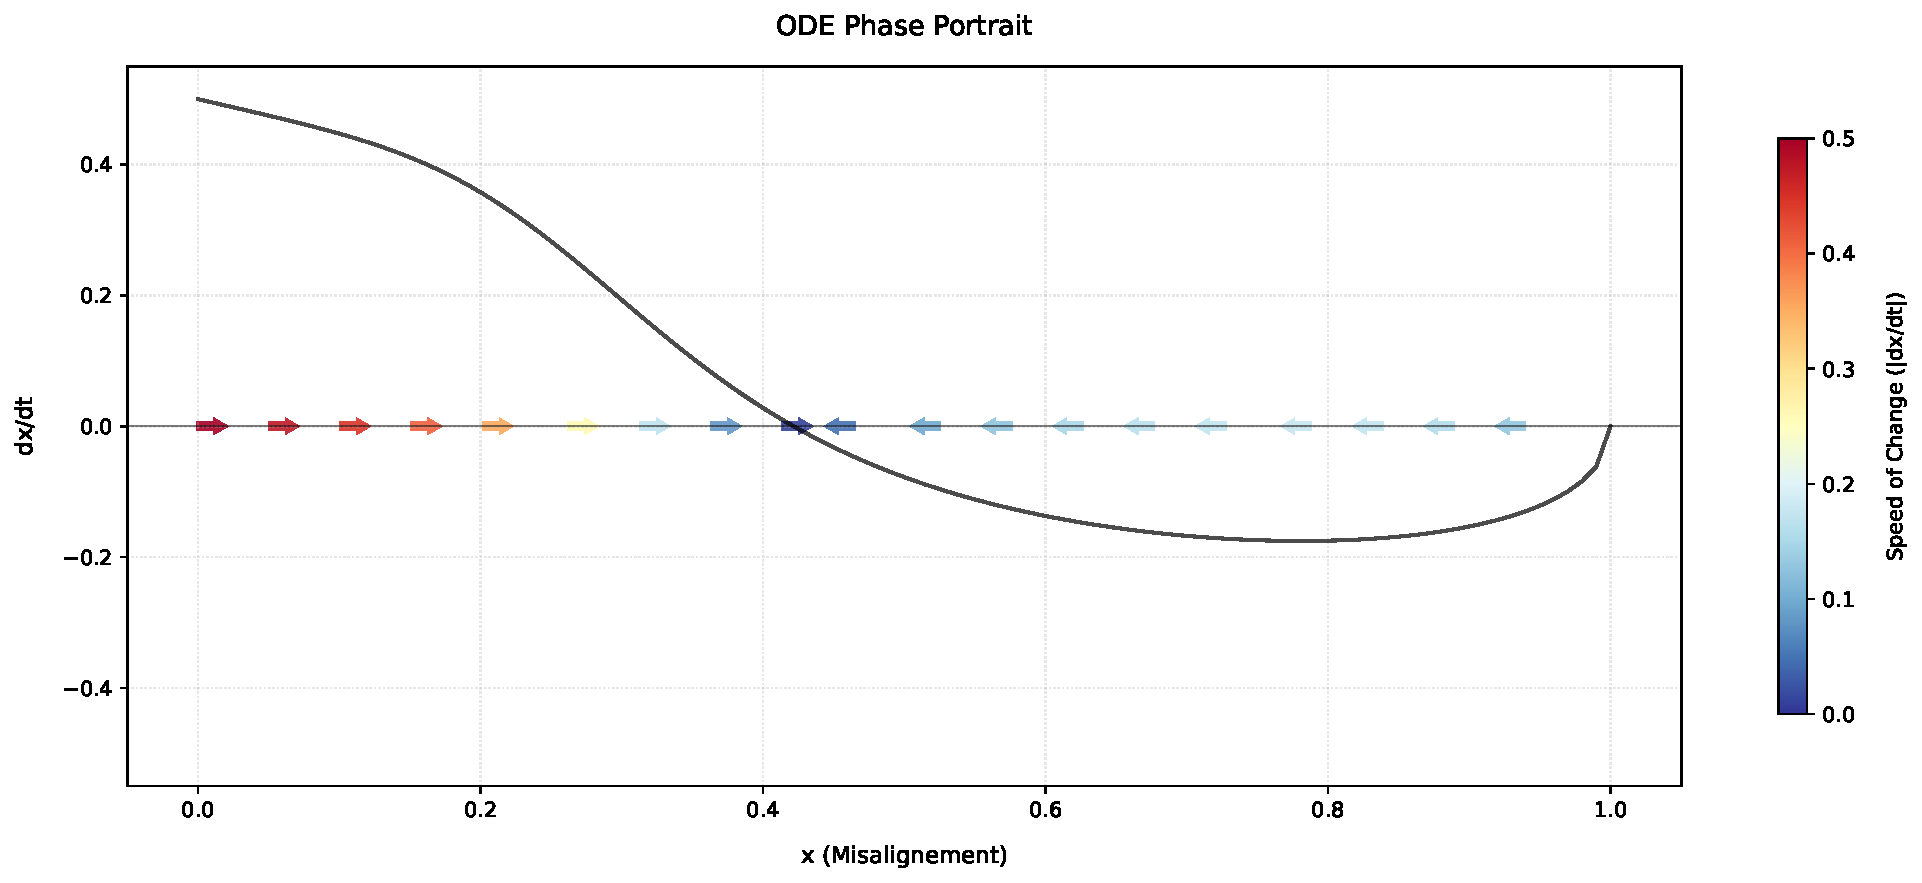
\includegraphics[width=0.9\textwidth]{../images/results/phase-portrait.pdf}
	\caption{Phase portrait ($d = 0.5$, $a = 2$, $h = 1$, $g = 0.5$, $r = 0.3$, $s = 3$)}
	\label{fig:phase_portrait}
\end{figure}

\subsubsection{Bifurcation Diagram and Lyapunov exponent}
Users can select any parameter for the x-axis via a dropdown menu and focus on specific ranges of interest.
Adjust the sliders, and you may get the chacteristic period-doubling bifurcations and the emergance of chaotic behaviour.

\textbf{Pro tip:} Set $h$ (IT rigidity) to a low value for observing beatiful patterns.

\begin{figure}[H]
	\centering
	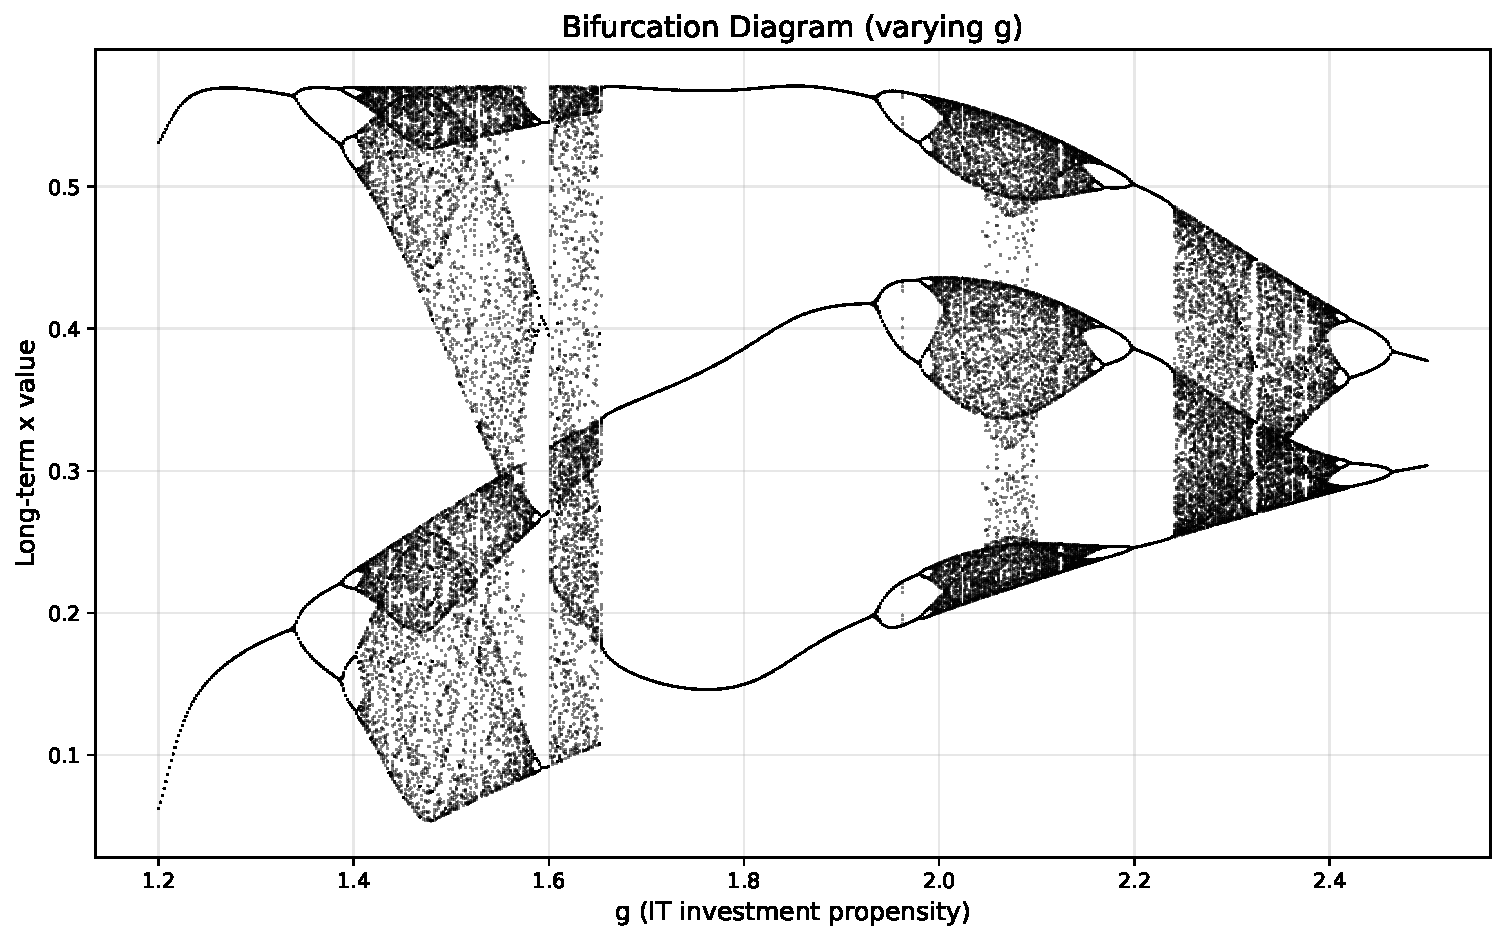
\includegraphics[width=0.8\textwidth]{../images/results/big-diagram.pdf}
	\caption{Shouldn't this be exposed at Louvre? ($d = 0.5$, $a = 7$, $h = 0.3$, $r = 0.3$, $s = 5.1$)}
	\label{fig:bifurcation}
\end{figure}

The \textbf{Lyapunov exponent} ($\lambda$) quantifies the rate of separation of infinitesimally close trajectories in a dynamical system. For a 1D map $x_{n+1} = f(x_n)$, it's calculated as:

\begin{equation}
\lambda = \lim_{N \to \infty} \frac{1}{N} \sum_{n=0}^{N-1} \ln |f'(x_n)|
\end{equation}

\begin{itemize}
    \item $\lambda > 0$: Chaotic behavior (exponential divergence)
    \item $\lambda = 0$: Neutral stability (periodic)
    \item $\lambda < 0$: Stable fixed point
\end{itemize}

\begin{figure}[H]
	\centering
	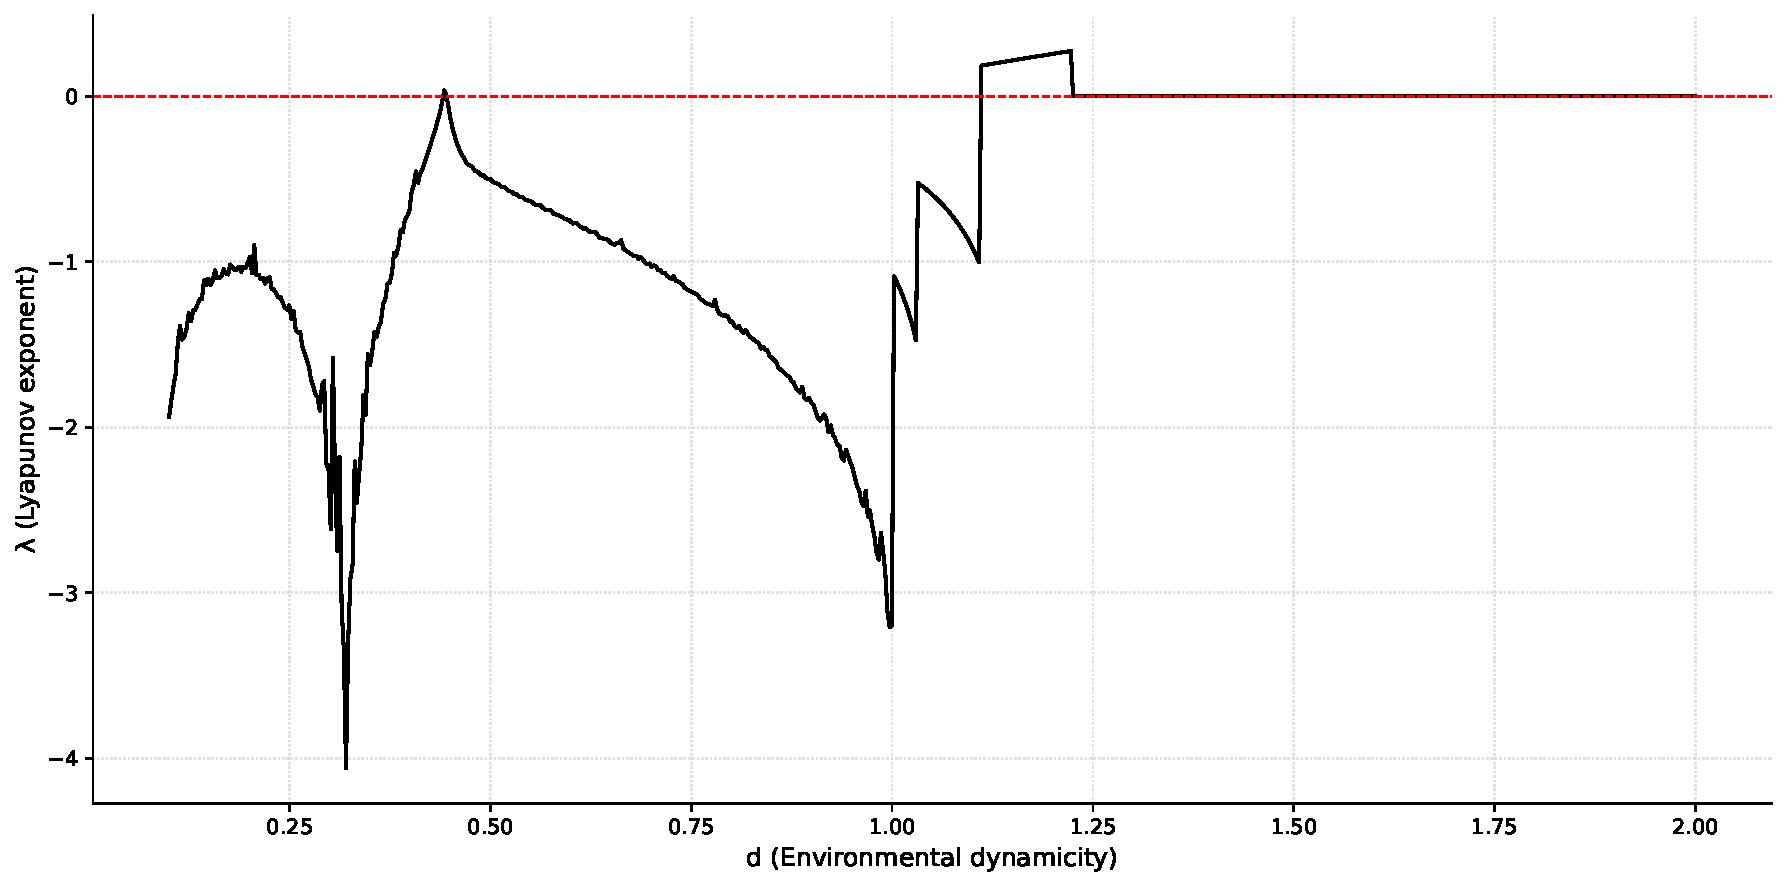
\includegraphics[width=0.8\textwidth]{../images/results/lyapunov.pdf}
	\caption{Chaotic behavior detected! ($x_0 = 0.3$, $a = 2.7$, $h = 0.32$, $g = 2.0$, $r = 0.3$, $s = 3.0$)}
	\label{fig:lyapunov}
\end{figure}

\clearpage

\subsection{Interesting Cases}
To enhance the user experience, I've included a couple noteworthy cases encopassing different system behaviors. Specifically, I analyzed and visualized first periodic then chaotic behavior, along with alignment as a function of parameter pairs.

\subsubsection{Alignment as a function of two parameters}
Find out how variations in pairs of parameters, such as a (efficiency) and h (rigidity), affect long-term alignment.

To explore this, I generated \textit{contour line plots} using a custom helper function, where the output is visualized both through \textbf{color gradients} and \textbf{contour lines}.
The x-axis represents the first parameter, and the y-axis the second. The function accepts a central value and range for each parameter, then simulates outcomes over a grid to compute equilibrium alignment levels. This visual approach allows for an intuitive understanding of how each pair of parameters influences the system’s behavior.

The parameter pairs displayed below are: (a, h), (a, g), (h, g), and (r, s).

Let’s examine the first case as an example. From the plot, we can infer that improving efficiency (a↑) while reducing rigidity (h↓) decreases dissatisfaction, albeit with diminishing marginal returns.  
This is a pattern consistent with real-world IT system behavior.

\begin{figure}[h]
    \centering
    \begin{minipage}[b]{0.48\textwidth}
        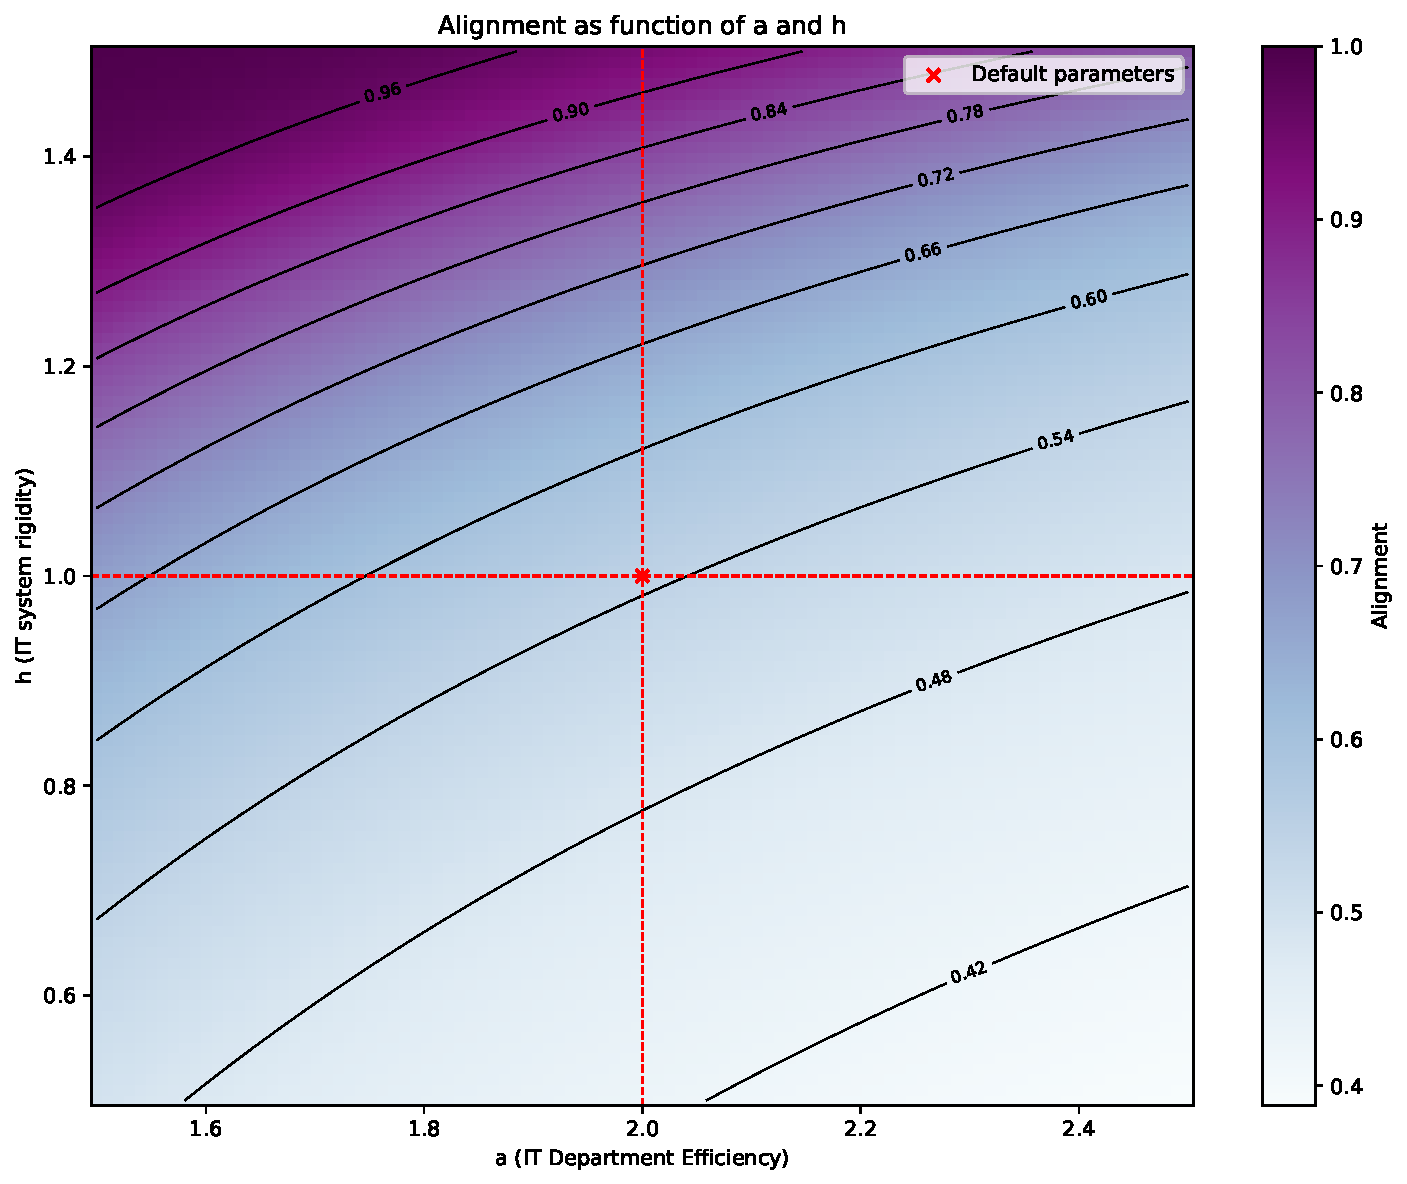
\includegraphics[width=\textwidth]{../images/int-cases/sim-1.pdf}
    \end{minipage}
    \hfill
    \begin{minipage}[b]{0.48\textwidth}
        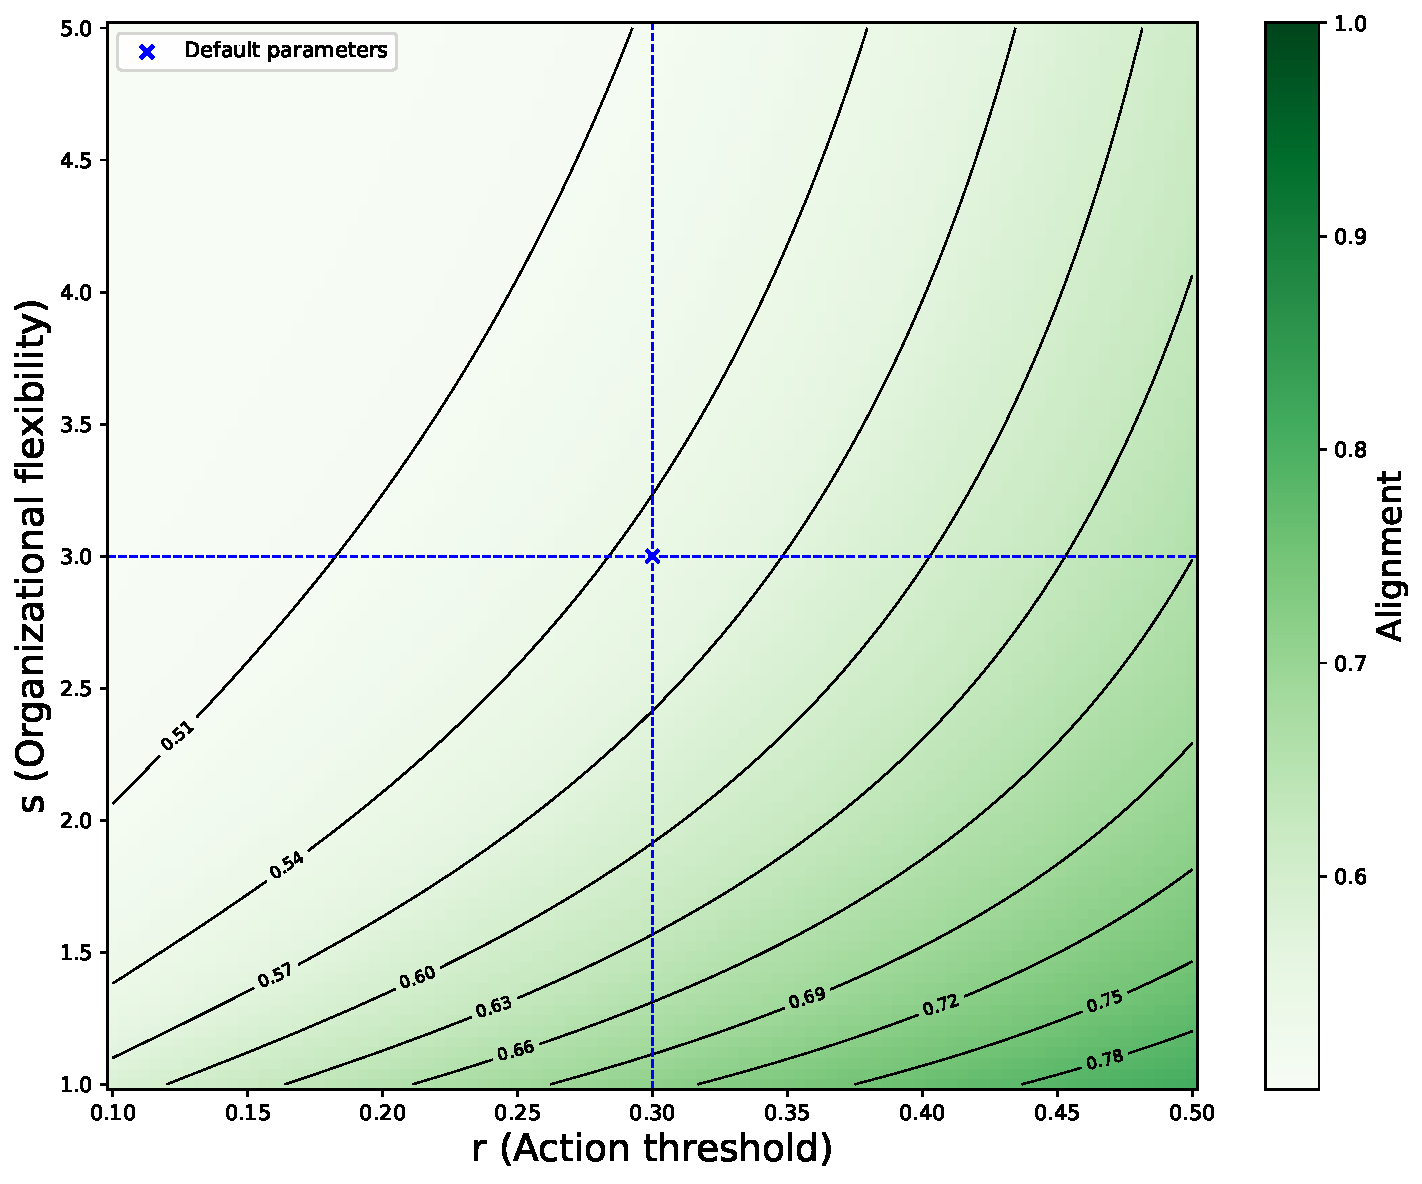
\includegraphics[width=\textwidth]{../images/int-cases/sim-2.pdf}
    \end{minipage}
    \par\vspace{1em}
    \begin{minipage}[b]{0.48\textwidth}
        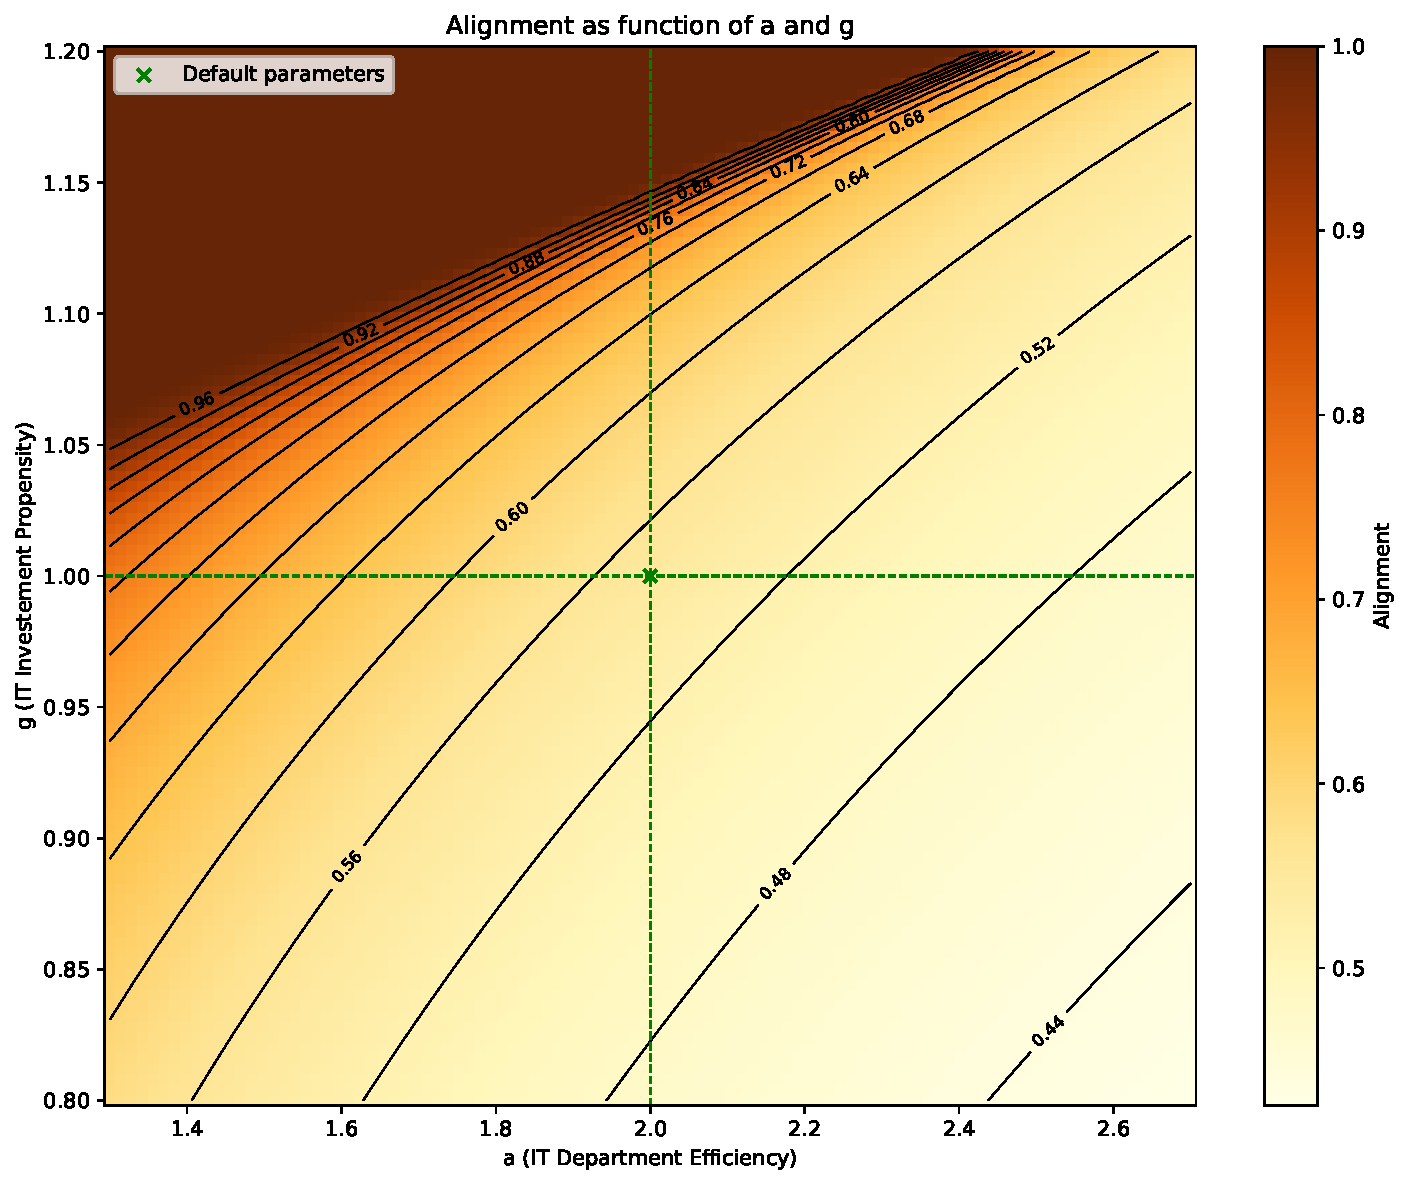
\includegraphics[width=\textwidth]{../images/int-cases/sim-3.pdf}
    \end{minipage}
    \hfill
    \begin{minipage}[b]{0.48\textwidth}
        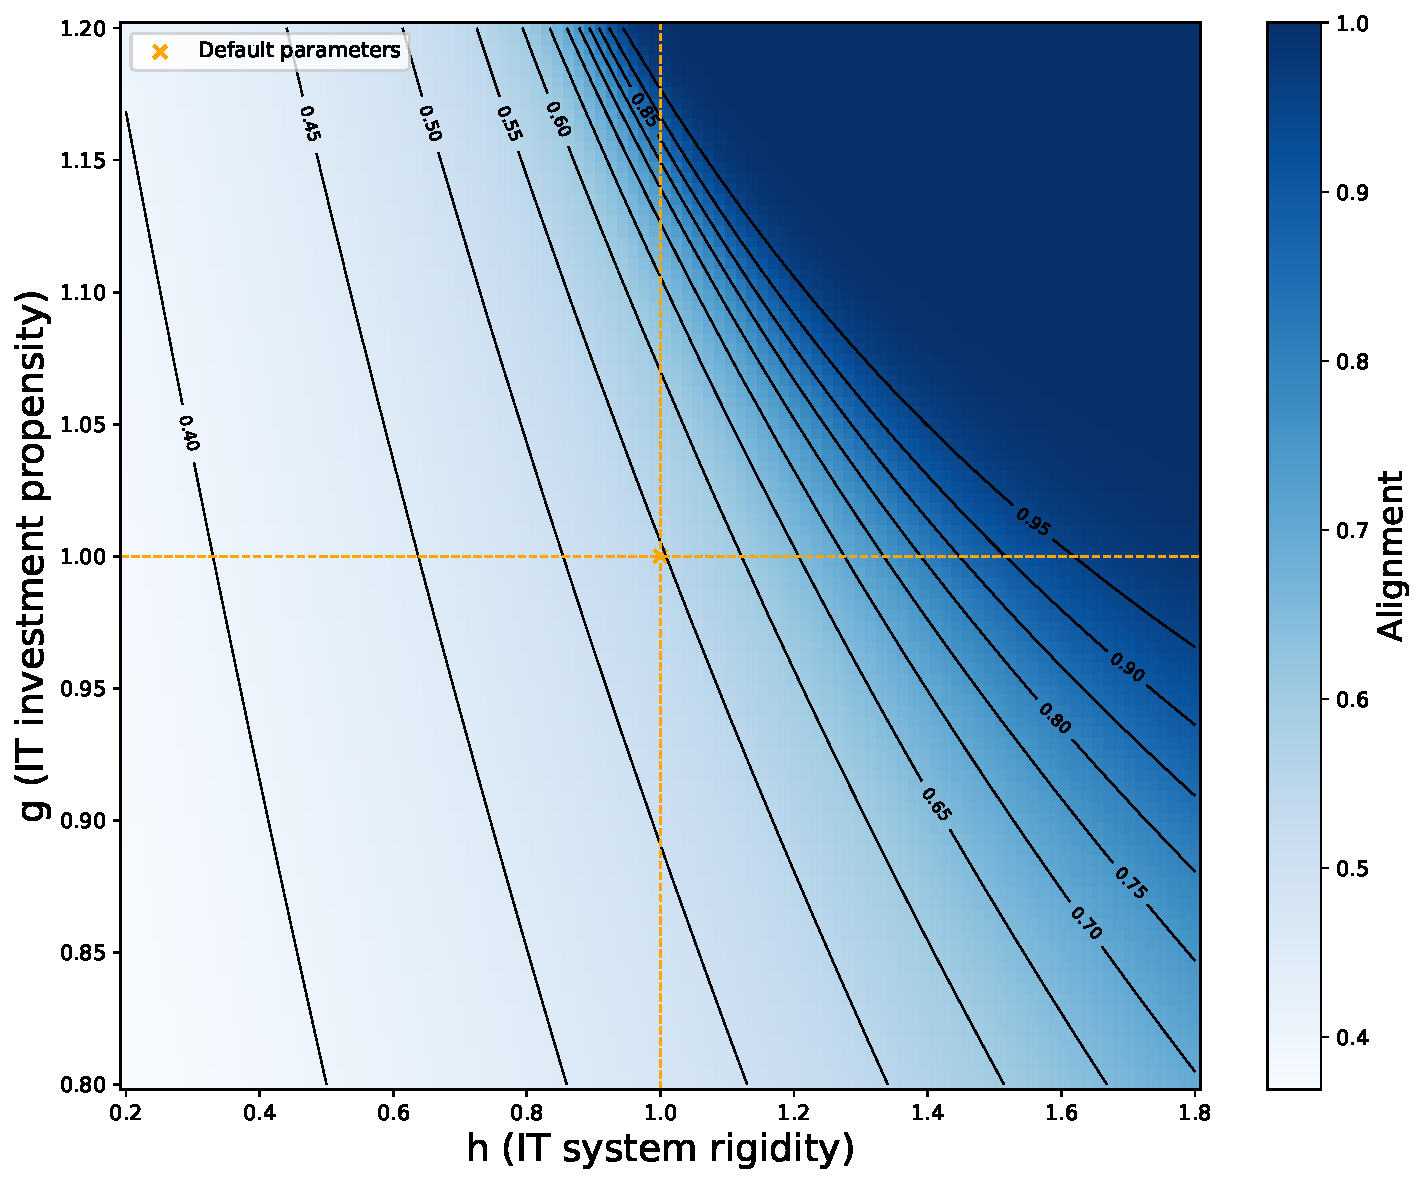
\includegraphics[width=\textwidth]{../images/int-cases/sim-4.pdf}
    \end{minipage}
    \caption{Contour plots showing alignment as a function of different parameter pairs.}
    \label{fig:alignment-contour-plots}
\end{figure}

\clearpage
\subsubsection{Periodic Behaviour}
Let's examine a parameter combination that produces stable \textbf{periodic} behaviour:

\begin{verbatim}
{"x0": 0.3, "d": 0.3, "a": 4.0, "h": 0.4, "g": 0.65, "r": 0.3, "s": 3.5}
\end{verbatim}

\begin{wrapfigure}[15]{r}{0.45\textwidth}
    \centering
    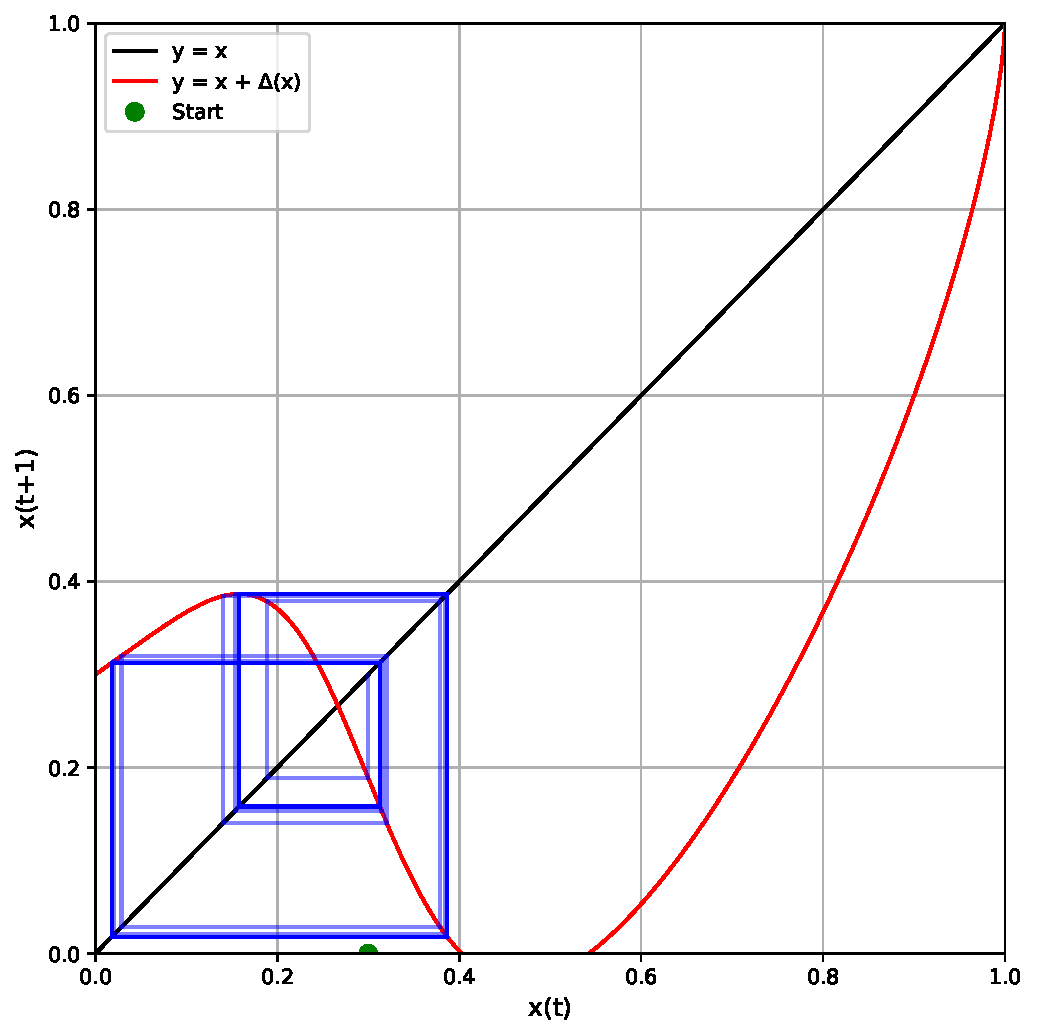
\includegraphics[width=0.45 \textwidth]{../images/int-cases/periodic-cobweb.pdf}
    \label{fig:periodic-cobweb}
\end{wrapfigure}

\RaggedRight

With this configuration:
\begin{itemize}
    \item Moderate environmental pressure ($d = 0.3$) prevents immediate convergence to full misalignment ($x=1$).
    \item Strong IT efficacy ($a = 4$) amplifies the $B(x)$ term's impact.
    \item Balanced organizational response ($s = 3.5$) creates sufficient feedback delay.
\end{itemize}

The system settles into a period-4 oscillation between approximately $[0.3127, 0.1583, 0.3869, 0.0181]$, as visible in the outputs:

\begin{itemize}
    \item The time evolution plot shows perfect repetition every 4 steps.
    \item The cobweb plot (right) reveals the characteristic "rectangle" pattern.
    \item The negative Lyapunov exponent ($-0.7598$) confirms stable periodicity.
\end{itemize}

\begin{figure}[h]
    \centering
    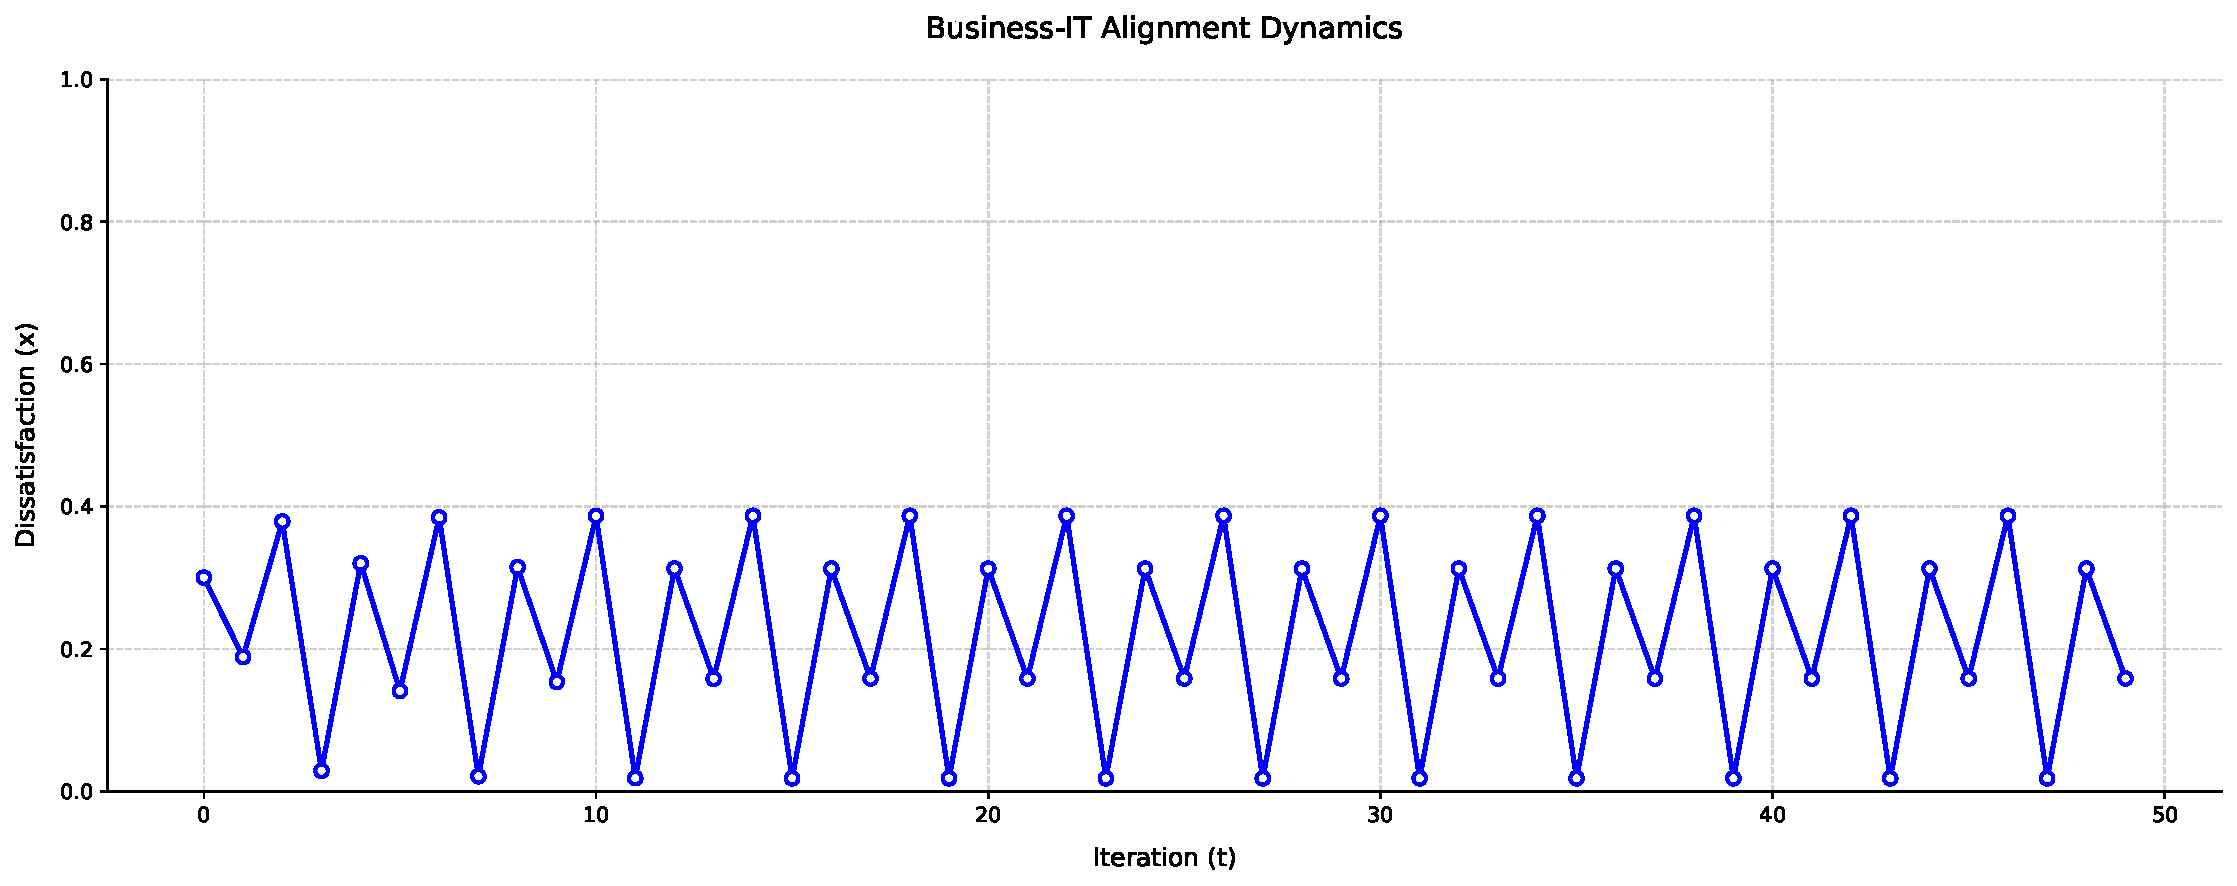
\includegraphics[width=0.9\textwidth]{../images/int-cases/periodic-long-term.pdf}
    \label{fig:periodic-time}
\end{figure}

\subsubsection{Chaotic Behaviour}
Now it's time for some \textbf{chaos}! 
Let's vary the environmental dynamicity parameter $d$ between 0.1 and 2, while keeping other parameters fixed:

\begin{verbatim}
{"x0": 0.3, "a": 5.0, "h": 0.3, "g": 1, "r": 0.25, "s": 3.0}
\end{verbatim}

The resulting plots are wild. Here's what we see:
\begin{itemize}
    \item For low values of $d$, the system behaves fairly regularly. Except for a brief chaotic-looking window around $d=0.25$, it follows a classic period-doubling route to chaos, oscillating between 2, then 4, then 8 values, and so on. 
    \item Once $d$ passes about 0.6, things get truly chaotic. The long-term values of $x$ become unpredictable.
    \item After $d \approx 0.8$, chaotic behavior fades and we see what looks like reverse bifurcation, where multiple branches collapse back into fewer.
    \item For larger values ($d>1.1$), the system stabilizes completely. It settles into a single outcome, and by the end, all points collapse into a perfectly misaligned state.
\end{itemize}

This is confirmed by the Lyapunov Exponent:
\begin{itemize}
    \item When $\lambda<0$, nearby trajectories come together — this means the system is stable or periodic.
    \item When $\lambda>0$, small differences blow up over time — the signature of chaos. This happens mainly between $d \approx 0.6$ and $d \approx 1.5$, matching the chaotic zone from the bifurcation diagram.
    \item Sharp dips below zero show periodic windows — moments where order reappears inside the chaos.
    \item Toward the end, the Lyapunov exponent drops back to zero, confirming the system has returned to a fully stable state.
\end{itemize}

\begin{figure}[h]
    \centering
    \begin{subfigure}{0.48\textwidth}
        \centering
        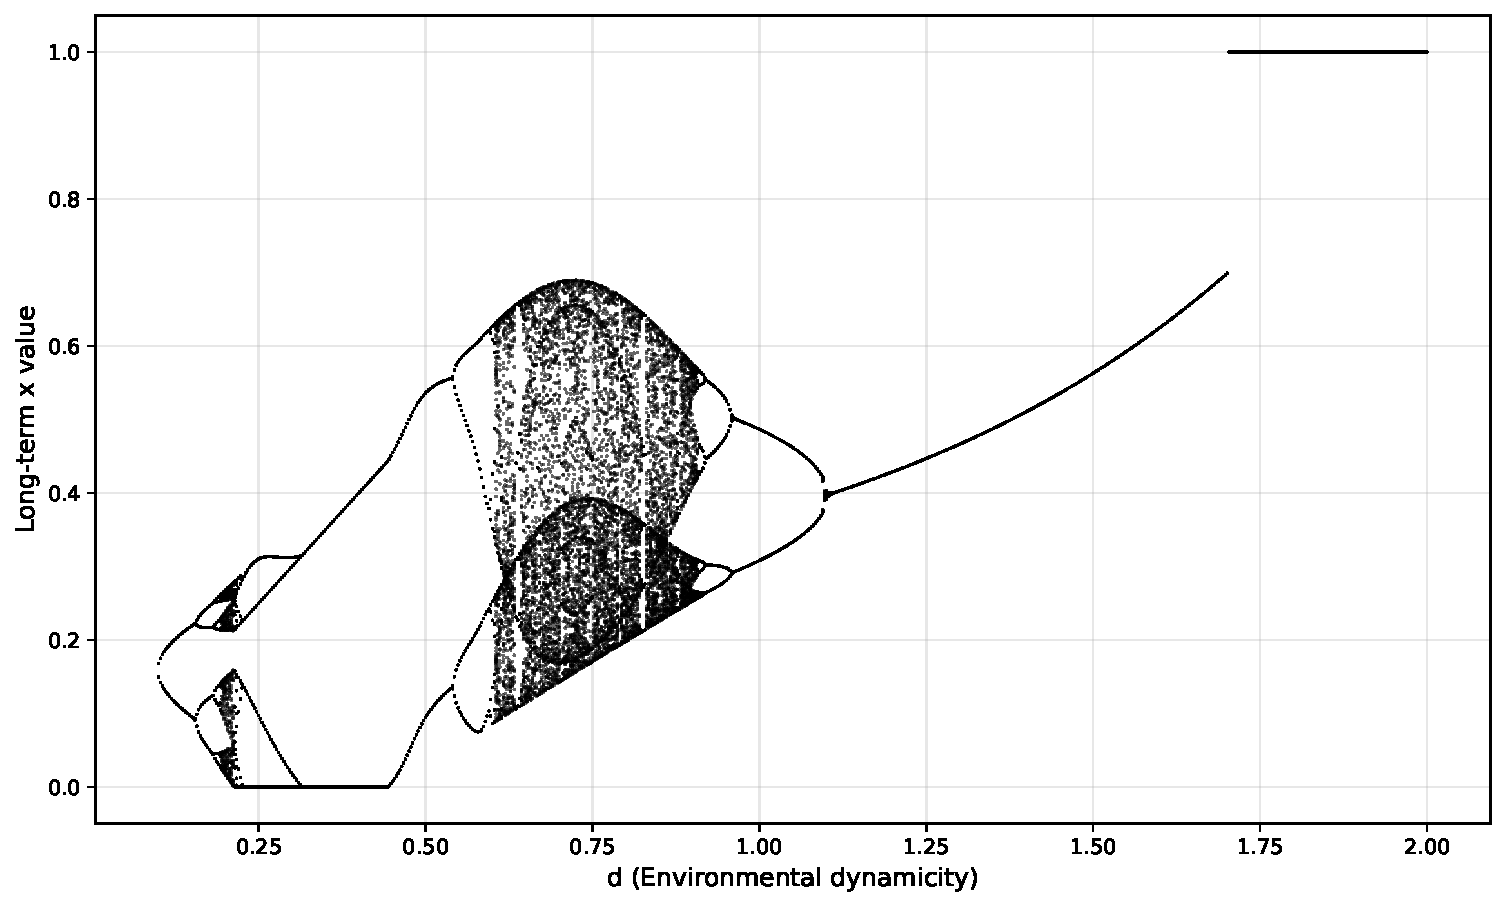
\includegraphics[width=\textwidth]{../images/int-cases/chaotic-bifurcation.pdf}
        \caption{Bifurcation diagram showing chaotic regions}
        \label{fig:chaotic-bifurcation}
    \end{subfigure}
    \hfill
    \begin{subfigure}{0.48\textwidth}
        \centering
        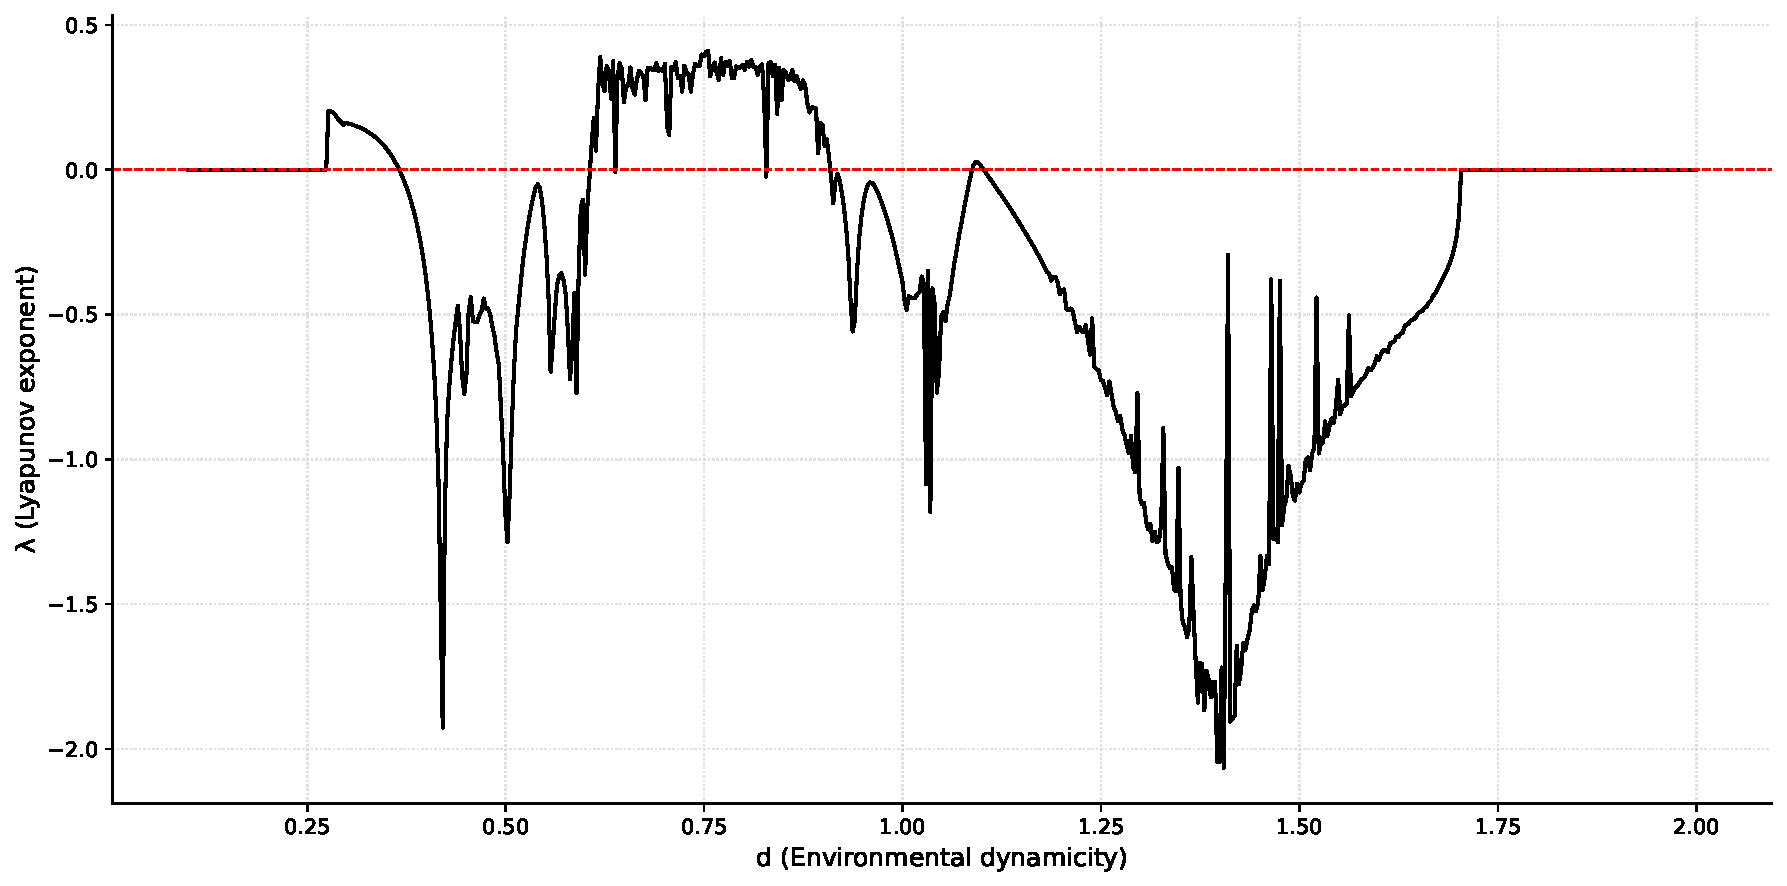
\includegraphics[width=\textwidth]{../images/int-cases/chaotic-lyapunov.pdf}
        \caption{Lyapunov exponent analysis}
        \label{fig:chaotic-lyapunov}
    \end{subfigure}
    \caption{Analysis of chaotic behavior through bifurcation and Lyapunov exponent}
    \label{fig:chaos-analysis}
\end{figure}

Let's take $d = 0.75$ and call \texttt{cobweb\_plot()}. Notice how messy the cobweb is!

\begin{figure}[h]
    \centering
    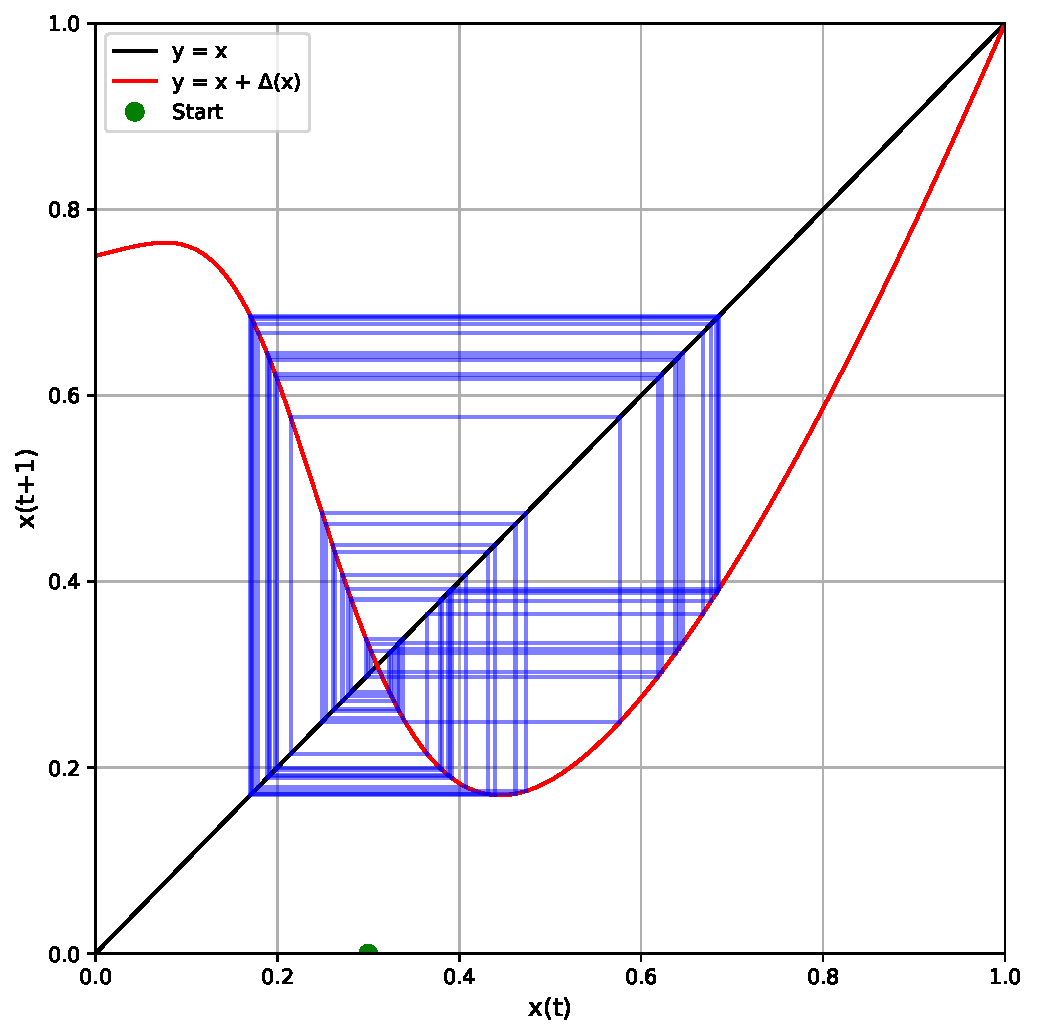
\includegraphics[width=0.6\textwidth]{../images/int-cases/chaotic-cobweb.pdf}
    \caption{Chaotic cobweb plot at $d=0.75$}
    \label{fig:chaotic-cobweb}
\end{figure}

\clearpage

\section{Personal Reflection}
Let me start by saying that I absolutely loved working on this project.

When I was assigned a discrete-time equation similar to the logistic map that could show different behaviors (chaotic, periodic, misaligned) depending on its initial conditions, I had only a vague idea of the underlying concepts. 
So I spent the first two weeks watching YouTube videos and I remember thinking: \textit{“What a bizarre corner of math I’ve stumbled into”}.

Once I had a solid grasp of what the equation represented and what its components meant, I started writing code. 
Using \texttt{matplotlib} and \texttt{ipywidgets} felt like the natural choice. They’re the go-to tools for this kind of interactive visualization. 
Honestly, coding wasn’t too difficult. Sure, I ran into some issues passing the selected parameter into the \texttt{update\_diagram\_function}, and calculating the Lyapunov exponent took some work.
But overall, things went smoothly. 

And that lack of major technical obstacles allowed me to focus on higher-level thinking which, in my opinion, is what data science should be about. 
You shouldn’t get bogged down in arrays, lambdas and method calls; the real focus should be on exploring and interpreting numbers. 
Because of that, I was able to experiment with sliders, explore visually stunning diagrams, test out a few interesting scenarios, and write down insights in the markdown cells as I went.

I’ve just enrolled in a double master’s program in Data Science, and I genuinely believe this field is the perfect blend of mathematics and computer science. Working on this project definitely played a role in my decision.

Collaborating directly with a professor was also a first for me. 
When someone you don’t know asks you to build a feature, it becomes clear how different their expectations and perspective might be from yours. 
It’s not always easy to satisfy the “customer”, but learning to navigate that dynamic was a valuable part of the experience.

However, what fascinated me most was learning that this equation models IT-business alignment. 
The parameters I labeled \texttt{d} and \texttt{r} — which I saw as just a sigmoid’s shape or a slope — were actually tied to company concepts like “environmental pressure” and “activation threshold.” 
That connection between math and the real world is incredible: you can describe the world using math and predict the future just by computing some numbers.

\textit{The hardest part of the project?} Screenshotting the interactive sliders. \newline
Since they’re not Matplotlib images, you can’t just export them to PDF. And LaTeX handles \texttt{.png} and \texttt{.jpg} files in strange ways. I tried everything: AI image enhancers, command-line tools, browser screenshots, converting to HTML. Nothing worked. 
After multiple failed attempts, I gave up. In the final report, the screenshots look a bit blurry. I guess the only real solution is to run the notebook and view the \texttt{ipywidgets} live.

\begin{thebibliography}{9}
	\bibitem{veritasium}
    Veritasium. (2020, January 29). \href{https://www.veritasium.com/videos/2020/1/29/this-equation-will-change-how-you-see-the-world}{This Equation Will Change How You See the World}.

	\bibitem{chaos}
	Strogatz, S. H. (2018). \textit{Nonlinear dynamics and chaos: with applications to physics, biology, chemistry, and engineering}. CRC Press.

	\bibitem{italign}
	Luftman, J. (2003). \textit{Assessing IT/business alignment}. Information Systems Management, 20(4), 9-15.
\end{thebibliography}

\appendix
\section{Appendix: Complete Python Code}
The full implementation is available at: \url{https://github.com/Kinshale/pii}

\end{document}
